\documentclass[a4paper,12pt]{article}

\usepackage[utf8]{inputenc}
\usepackage{listings}
\usepackage{color}
\usepackage{polski}
\usepackage[T1]{fontenc}

\usepackage{graphicx} 
\usepackage[export]{adjustbox}
\usepackage{wrapfig} 
\usepackage{subcaption}
\usepackage{amssymb}
\usepackage{setspace}
\usepackage{datetime}
\usepackage{mathptmx}
\usepackage{tocloft}
\usepackage{blindtext}
\usepackage{hyperref}

\definecolor{javared}{rgb}{0.6,0,0} % for strings
\definecolor{javagreen}{rgb}{0.25,0.5,0.35} % comments
\definecolor{javapurple}{rgb}{0.5,0,0.35} % keywords
\definecolor{javadocblue}{rgb}{0.25,0.35,0.75} % javadoc

\lstdefinestyle{mystyle}{
    basicstyle=\linespread{1}\small\ttfamily,
    backgroundcolor=\color{white},   
    breakatwhitespace=false,         
    breaklines=false,                 
    captionpos=b,                    
    commentstyle=\color{javagreen},   
    escapeinside={\%*}{*)},          
    extendedchars=false,             
    keepspaces=true,                
    keywordstyle=\color{javapurple}\bfseries,
    morecomment=[s][\color{javadocblue}]{/**}{*/},
    language=Java,                
    numbers=left,                    
    numbersep=7pt,                  
    numberstyle=\tiny\color{black}, 
    rulecolor=\color{black},         
    showspaces=false,                
    showstringspaces=false,        
    showtabs=false,                  
    stepnumber=1,                  
    stringstyle=\color{javared},     
    tabsize=2,	                   
    title=\lstname,
    columns=flexible
}
%frame=single,	               
%basicstyle=\footnotesize,
\lstset{style=mystyle}

\urlstyle{
    colorlinks=true,
    linkcolor=blue,
    filecolor=magenta,      
    urlcolor=cyan,
    pdftitle={Sharelatex Example},
    bookmarks=true,
    pdfpagemode=FullScreen,
}

\newcommand{\MONTH}{%
  \ifcase\the\month
  \or Styczeń % 1
  \or Luty % 2
  \or Marzec % 3
  \or Kwiecień % 4
  \or Maj % 5
  \or Czerwiec % 6
  \or Lipiec % 7
  \or Sierpień % 8
  \or Wrzesień % 9
  \or Październik % 10
  \or Listopad % 11
  \or Grudzień % 12
  \fi
}
\makeatletter
\newcommand\spacingInSimpleItemize{0.8}
\newcommand\spacingInSolemnItemize{1.2}
\newcommand{\YEAR}{\@Roman{\the\year}}
\makeatother

\usepackage[left=2.5cm, right=2.5cm, top=2.5cm, bottom=2cm]{geometry}
\setlength{\parindent}{4em}
\setlength{\parskip}{1pt}
\renewcommand{\baselinestretch}{1.5}
\renewcommand{\cftsecleader}{\cftdotfill{\cftdotsep}}
%?
\usepackage[11pt]{moresize}
\prefixing

\author{Przemysław Woldon}
\date{}

\begin{document}
    %strona tytułowa
    \begingroup
        \fontsize{12pt}{0.2}\selectfont
            \begin{center}Politechnika Łódzka\end{center}
            \begin{center}Wydział Elektrotechniki, Elektroniki, Informatyki i Automatyki\end{center} 
            \begin{center}Instytut Informatyki Stosowanej\end{center} 
        \vspace*{125px}     
        \fontsize{14pt}{0.2}\selectfont
            \begin{center}\textbf{PRACA DYPLOMOWA INŻYNIERSKA}\end{center} 
        \vspace*{50px}
        \fontsize{12pt}{0.2}\selectfont
            \begin{center}System umożliwiający digitalizację zapisów nutowych pieśni, \\\vspace{3mm} ułatwiający ich przechowywanie i przetwarzani\end{center} \vspace{5mm}
            \begin{center}A system for digitization of sheet music facilitating their storage and processing\end{center} 
        \vspace*{50px}
        \fontsize{12pt}{0.2}\selectfont 
            \begin{center}Przemysław Woldon\end{center} 
            \begin{center}Numer albumu: 195092\end{center} 
        \vspace*{70px}
        \fontsize{12pt}{0.2}\selectfont 
            \begin{flushright}Opiekun pracy:\end{flushright} 
            \begin{flushright}Dr. inż. Paweł Kapusta\end{flushright} 
        \vspace*{90px}
        \fontsize{12pt}{0.2}\selectfont 
            \begin{center}Łódź, \MONTH \vspace{2cm}  \the\year \end{center} 
    \endgroup
	\newpage
	
	\pagenumbering{gobble}
    \pagenumbering{arabic}
	\setcounter{page}{2}
    \tableofcontents
	\newpage 
	
    \section*{Streszczenie}
	\addcontentsline{toc}{section}{Streszczenie}
	    \paragraph{\indent} Niniejsza praca dyplomowa w sposób            najzwięźlejszy opisuje prototyp systemu umożliwiającego       pozyskanie tekstu z obrazów stron śpiewników kościelnych i     jego dalsze możliwości rozwoju.
        \par Na pracę pisemną składają się dwie zasadnicze części:        teoretyczna i praktyczna. Część teoretyczna opisuje           wybrane technologie, które zostały wykorzystane w             systemie. Zaś część praktyczna w sposób przejrzysty           przedstawia zaimplementowane algorytmy. W podsumowaniu        autor w sposób krytyczny rekapituluje wykonaną pracę          zwracając uwagę na zalety i wady wypracowanego                rozwiązania, jednocześnie podając sposoby na rozwiązanie      powstałych problemów oraz wskazuje, proponuje drogi           rozwoju projektu.   
	\section*{Abstract}
    \addcontentsline{toc}{section}{Abstract}    
	\newpage 

	\section{Wstęp}
		\paragraph{\indent} Cyfryzacja dotyka wielu obszarów naszego       życia. Jednym z nich jest sztuka (w tym muzyka, muzyka        sakralna). Obecnie coraz częściej w świątyniach możemy        spotkać się z rzutnikami lub wyświetlaczami led, 
			na których ekranizowane są teksty pieśni. Cyfrowe zbiory pieśni dostarczane przez producentów wyświetlaczy 
			nie są w stanie sprostać wymaganiom jakie stawia przed nimi: dynamiczny rozwój muzyki --- powstawaniu nowych utworów, 
			zróżnicowanym tradycjom lokalnym oraz indywidualnym upodobaniom muzyków kościelnych wykorzystującym różne śpiewniki. 
			Czasochłonny proces budowy wspomnianych zbiorów często polega na ręcznym przepisywaniu tekstów pieśni 
			z wykorzystywanych przez muzyków kościelnych śpiewników. Automatyzacja tego procesu pozwoli na łatwiejsze dopasowanie zbiorów 
			do potrzeb muzyków kościelnych i tradycji lokalnych. 
	        Przed przystąpieniem do prac nad aplikacją autor nie      spotkał się z wykorzystaniem na rynku polskim             oprogramowania rozwiązującego powyższe problemy.
		\par Dzięki pracy nad tą aplikacją autor mógł połączyć swoje dwie pasje --- muzykę kościelną i informatykę. 
			Pomysł budowy aplikacji narodził się z zaobserwowania, że osoby odpowiedzialne za muzykę kościelna przeznaczają znaczącą liczbę godzin 
			na ręczne przepisywanie śpiewników, poprawę błędów w już dostarczonych zbiorach. Zaangażowanie technik informatycznych do tego zadania 
	        umożliwi szybszą budowę własnych zbiorów pieśni.  
			Budowa prototypu zapewniającego pełną funkcjonalność,  daje możliwość jego opublikowania 
			i dotarcia do szerokiego grona interesariuszy, \textbf{co może stanowić punkt wyjściowy do dalszych prac nad aplikacją tak aby wypracowane rozwiązanie było użyteczne, niezawodne, wydajne i wspierane.}
		
		\subsection{Cel pracy}
			\paragraph{\indent} Celem niniejszej pracy dyplomowej było skonstruowanie algorytmów przetwarzających strony śpiewników kościelnych tak, 
				aby jak najlepiej przygotować je do optycznego rozpoznania zawartego w nich tekstu. W algorytmach wykorzystane zostały metody przetwarzania obrazów, 
				które redukują szumy, usuwają obszary, które nie zawierają znaczących w analizie danych (eliminacja nadmiarowych informacji), 
				prostują strony, wykrywają i usuwają znaki muzyczne, wykrywają znaki (cyfry, litery, znaki interpunkcyjne), 
				zaś algorytmy cyfrowego rozpoznawania tekstu odczytują wykryte litery uwzględniając polskie znaki diakrytyczne. 
				Dzieki zastosowaniu konwolucyjnych sieci neuronowych wypracowane rozwiąznie zostało uogólnione, a finalne algorytmy umożliwiają pracę 
				na różnych danych wejściowych. Zaś budowa aplikacji uwzględniająca dobre praktyki programowania ułatwi jej dalszy rozwój. 
	\newpage 

	\section{Wykorzystane technologie}
	    \paragraph{\indent} Cyfrowe przetwarzanie obrazów \textit{(ang. digital image processing)} jest dziedziną nauki 
			zajmującą się reprezentacją obrazu w pamięci komutera, jego akwizycją i przetwarzaniem. 
        \par Obecnie dostępnych jest wiele bibliotek umożliwiających pracę z obrazami, na przykład: Imagemagick, Generic Image Library, SIMD i inne. 
			Najbardziej powszechną biblioteką jest bilbioteka OpenCv, dostarcza ona bardzo bogatą, bezkonkurencyjną funkcjonalność, przejrzystą 
			i zawierającą podstawy matematyczne dokumentację, zaś dynamicznie rozwijająca się społeczność zgromadzona wokół biblioteki ułatwia 
			z nią pracę szczególnie nowym użytkownikom.
	    
		\subsection{Biblioteka OpenCv}
			%\paragraph{\indent} 
			%	OpenCv jest biblioteką służącą do komputerowego przetwarzania obrazów oraz uczenia maszynowego, o otwartym kodzie źródłowym.
		\subsubsection{Zarys historyczny}
			\paragraph{\indent} Prace nad budową tej biblioteki rozpoczął jeden z pracowników firmy Intel --- Gary Rost Bradski, 
				zainspirowany środowiskiem akademickim, które wówczas posiadało bardzo bogatą infrastrukturę służącą do przetwarzania obrazów, 
				jednak przeznaczoną dla użytku wewnętrznego. Studenci w obrębie jednej jednostki akademickiej dzielili się kodem zawierającym gotowe 
				implementacje algorytmów, co znacząco ułatwiało prace przy własnych projektach czy aplikacjach. Stąd głównym celem biblioteki OpenCv 
				jest udostępnienie wszystkim zainteresowanym zagadnieniami przetwarzania obrazów i sztucznej inteligencji gotowej, jednolitej, 
				darmowej infrastruktury pozwalającej na pracę, tak aby nie trzeba było ponownie "wynajdywać koła".
			\par OpenCv zostało przedstawione po raz pierwszy w 1999 roku szerszemu gronu odbiorców. 
			\par W wersji 1.0 kod biblioteki stanowiły wyłącznie najbardziej użyteczne przy przetwarzaniu obrazów algorytmy zaimplementowane w języku C. 
				Od tego czasu biblioteka znacząco się zmieniła. 
			\par W wersji 2.0 znaczący wpływ na wydanie wywarły trendy obecne w prowadzeniu projektów, w których wytwarza się oprogramowanie --- repozytorium kodu
				w systemie kontroli wersji Git, gdzie możemy znaleźć najnowszą wersję biblioteki i najświeższe poprawki, testy jednostkowe czy booty ciągłej kompilacji. 
				Zaimplementowano również interfejsy dla języków programowania takich jak C++ oraz Javy, Python’a, MATLAB---a. Od tego czasu nowe typy danych 
				i funkcje metody implementowano w C++, a już napisane w języku C dopasowano do nowej technologii. 
			\par Nieustannie zwiększająca się liczba zaimplementowanych algorytmów użytecznych przy przetwarzaniu obrazów przyczyniła się do modułowej budowy 
				biblioteki w wersji 3.0, która przedstawia się w sposób następujący:
                
                \begin{spacing}{\spacingInSimpleItemize}
    				\begin{itemize}
    					\item (warstwa wierzchnia) system operacyjny,
    					\item interfejsy dla różnych języków i aplikacje,
    					\item moduł \textit {opencv\_contrib} zawierający kod napisany i dołączony do biblioteki przez użytkowników,
    					\item rdzeń OpenCv,
    					\item optymalizacje sprzętowe (warstwa HAL \textit {ang. hardware acceleration layer}).
    				\end{itemize} 
                \end{spacing}
            
				\begin{figure}[!ht]  
					\begin{center}
						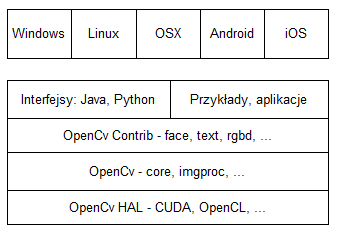
\includegraphics[width=12cm] {image//openCvBudowa.png} 
					\end{center}
					\caption
					    [Budowa modułowa OpenCv]
					    {Budowa modułowa OpenCv}
				\end{figure}

				\par OpenCv w tej wersji wspiera budowanie i dołączanie do biblioteki własnych modułów.
	            \newpage
				\begin{figure}[!ht]   
					\begin{center}
		    				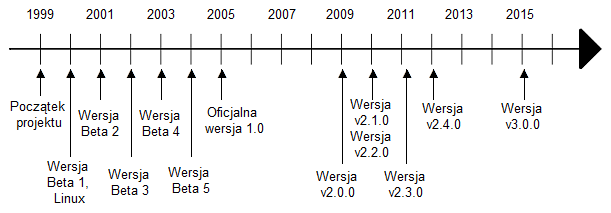
\includegraphics[width=\linewidth] {image//osCzasu.png} 
					\end{center}
					\caption
					    [Rozwój projektu w czasie]  
					    {Rozwój projektu w czasie}  
				\end{figure}


		\subsubsection{Popularność projektu}  
			\paragraph{\indent} Projekt cieszy się bardzo dużym powodzeniem, które nieustannie rośnie. Świadczy o tym liczba pobrań 
				wynosząca około 14 milionów razy, zaś miesięcznie około 200 tysięcy. Obecnie biblioteka zawiera ponad 2500 zoptymalizowanych algorytmów, 
				które służą do przetwarzania obrazów również w czasie rzeczywistym i uczenia maszynowego, co znacząco ułatwia tworzenie aplikacji użytkownikom. 
				Programiści piszący kod uwzględniali wymóg przenośności OpenCv, a więc możliwości kompilacji na każdym odpowiednim kompilatorze języka C++, 
				co wymusiło restrykcyjną zgodność ze standardem i ułatwiło obsługę różnych platform. Biblioteka dostępna jest na systemach operacyjnych takich jak: 
				Windows, Linux, Mac OS X, do których dołączyły systemy operacyjne platform mobilnych (Android i iOS), co znacząco przyczyniło się do zwiększenia liczby użytkowników.

		\subsubsection{Zastosowania biblioteki OpenCv}
			\paragraph{\indent} Dynamiczny rozwój technologiczny otwiera przed biblioteką nowy horyzont użyteczności. 
				OpenCv znajduje zastosowanie w wielu obszarach życia do tego stopnia że wykorzystanie projektu wydaje się rzeczą całkowicie naturalna,
				a wręcz niezauważalną. Biblioteka wykorzystywana jest w:
			
			    \begin{spacing}{\spacingInSimpleItemize}
			        \begin{itemize}
        				\item skanowaniu kodów QR,
        				\item monitoringu,
        				\item rozpoznawaniu dzwięków i muzyki,
        				\item obrazowaniu medycznym,
        				\item robotyce,	
        				\item przemyśle --- produkcji masowej i kontroli jakości,
        				\item wojsku --- bezzałogowe pojazdy, fotografie lotnicze,
				        \item analizie obiektów,
				        \item Google Street View
		            \end{itemize}
                \end{spacing}
    
    	\subsubsection{Reprezentacja obrazów}
			\paragraph{\indent} Obrazy można podzielić w najprostszy sposób na obrazy barwne i obrazy w skali szarości. Obrazy w bibliotece OpenCv 
				reprezentowane są w postaci macierzy (Mat). Narzędzie to udostępnia bogatą gamę możliwości reprezentacji poszczególnego piksela, 
				a więc i samego obrazu. Tak więc jeden piksel jest reprezentowany w następujący sposób --- CV\_xCy
			
				\begin{spacing}{\spacingInSimpleItemize}
					\begin{itemize}
						\item{x --- parametr określający typ}
							\begin{itemize}
								\item{8U --- 8---bitowy char bez znaku}
								\item{16S --- 16---bitowy short ze znakiem}
								\item{16U --- 16---bitowy short bez znakiu}
								\item{32S --- 32---bitowa liczba całkowita ze znakiem}
								\item{32F --- 32---bitowa liczba zmiennoprzecinkowa}
								\item{64F --- 64---bitowa liczba zmiennoprzecinkowa}
							\end{itemize}
						\item{y  --- parametr określający liczbę kanałów}
							\begin{itemize}
								\item{1 --- jeden kanał}
								\item{2 --- dwa kanały}
								\item{3 --- trzy kanały}
							\end{itemize}
					\end{itemize}	
				\end{spacing}
			
				lub jeśli użytkownik potrzebuje więcej kanałów może użyć funkcji CV\_xC(n), gdzie n --- liczba kanałów. Można również wybierać 
				z obfitej przestrzeni reprezentacji obrazu np. RGB, RGBA, HSV i innych. 
			\par Obrazy przechowywane jako pliki w pamięci komputera mają różne rozszerzenia, które wpływają na ich jakość, 
				wielkość zajmowanego miejsca na dysku. Przykładowe formaty obrazów: 
			
				\begin{spacing}{\spacingInSolemnItemize}
					\begin{itemize}
						\item TIFF \textit{(ang. Tagged---lmage File Format)} --- format standardowy i najbardziej podstawowy, używa algorytmu kompresji bezstratnej;
						\item JPEG \textit{(ang. Joint Photographic Experts Group)} --- używa algorytmu kompresji stratnej;
						\item PNG \textit{(ang. Portable Network Graphics)} --- używa algorytmu kompresji bezstratnej; 
						\item GIF \textit{(ang. Graphics Interchange Format)} --- używa algorytmu kompresji bezstratnej LZW \textit{(Lemple---Zif---Welch)}, 
							pliki mają małe rozmiary, często jest wykorzystywany do tworzenia animacji;
					\end{itemize}
				\end{spacing}
    
    \subsection{Konwolucyjne sieci neuronowe}
        \paragraph{\indent} Działanie sztucznych sieci neuronowych \textit{(Artificial neural network (ANN))} opiera się na modelu pojedynczego     
			neuronu (perceptronu), które zostają łączone w większe struktury. Matematyczną podstawę dla działania konwolucyjnych sieci neuronowych 
			\textit{(Convolutional neural networks (CNN))} stanowi splot (konwolucja) --- jest to operacja określana na dwóch funkcjach (np. f(t), g(t)) 
			w wyniku której otrzymujemy nową funkcję (np. h(t)); w przetwarzaniu obrazów jedną z funkcji jest analizowany obraz wejściowy, zaś druga filtr.
            Obraz wejściowy przechodzi przez wiele filtrów i każdy z nich mapuje cały obraz wejściowy biorac pod uwage jego części o rozmiarze filtra. 
			Tak wiec konwolucyjne sieci neuronowe uczą się obrazu, analizując go pewnymi wycinkami. Dokładnie filtr przechodzący przez obraz 
			mnoży odpowiednie wartości a następnie sumuje ich iloczyny.
        
            \begin{displaymath}
                h[m, n] = ( f \star g)[m, n] = \sum\limits_{j}\sum\limits_{k}f[j, k]g[m-j, n-k]
            \end{displaymath}
		    \newpage
		    
    	    \begin{figure}[h!]
                \centering
                \begin{subfigure}[b]{0.45\linewidth}
                    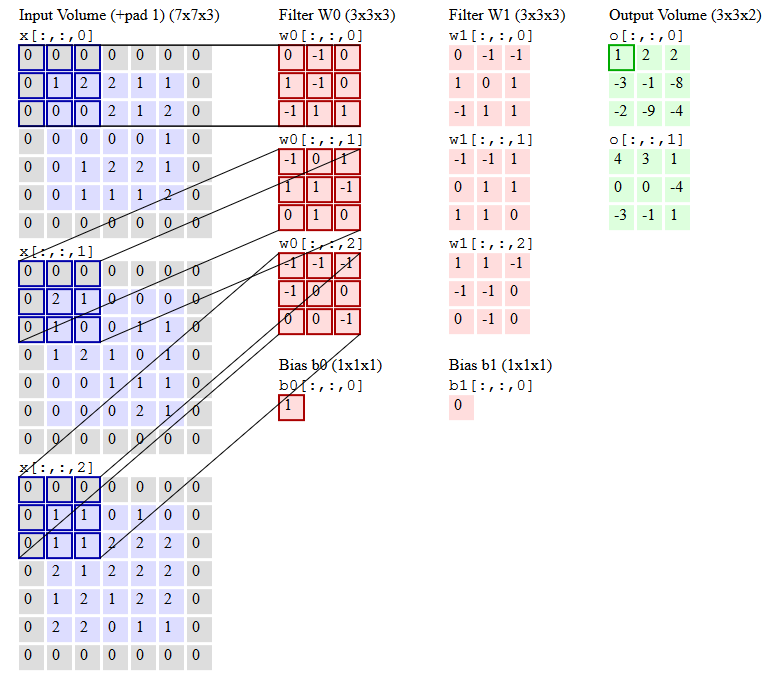
\includegraphics[width=\linewidth]{image//con_01.png}
					\caption{}
                \end{subfigure}
                \begin{subfigure}[b]{0.45\linewidth}
                    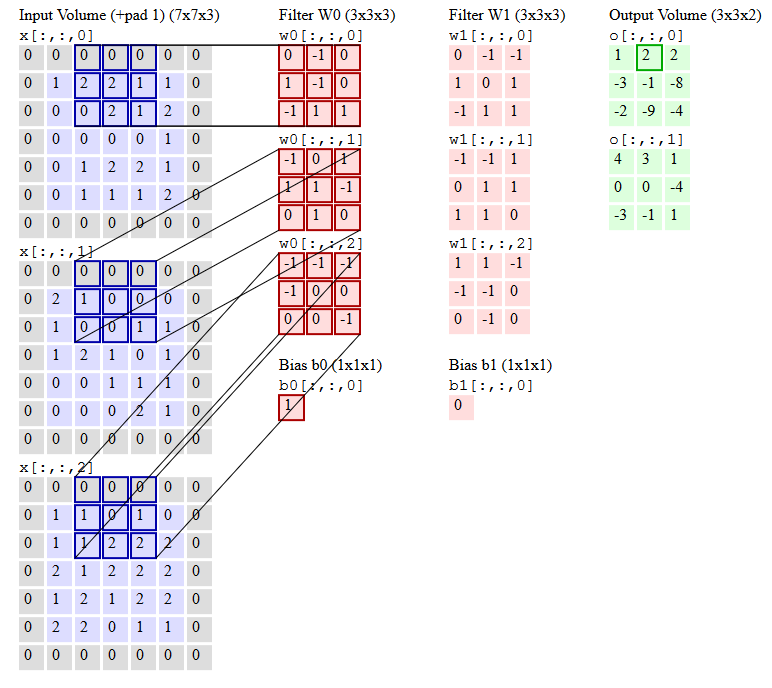
\includegraphics[width=\linewidth]{image//con_02.png}
					\caption{}
                \end{subfigure}
                \newline
                
				\begin{subfigure}[b]{0.45\linewidth}
                    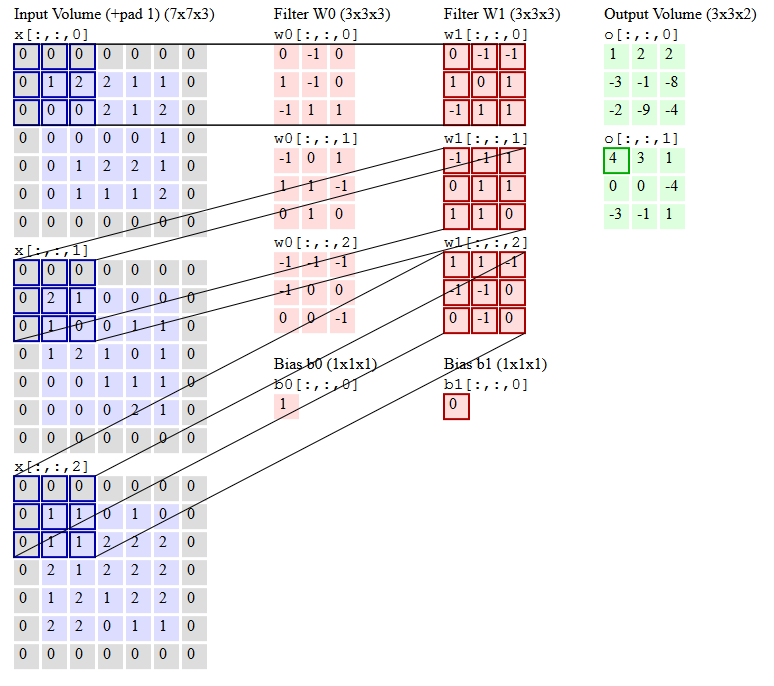
\includegraphics[width=\linewidth]{image//con_03.png}
					\caption{}
                \end{subfigure}
                \begin{subfigure}[b]{0.45\linewidth}
                    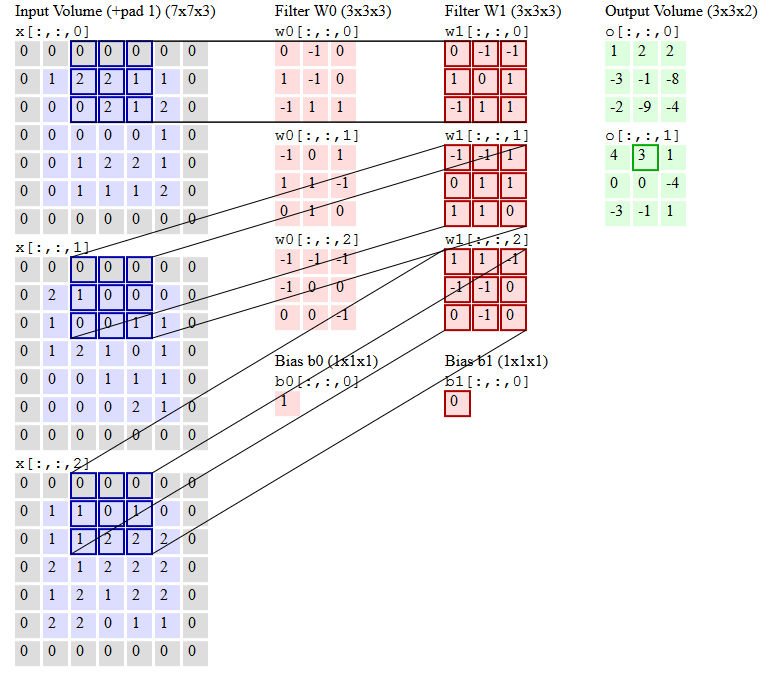
\includegraphics[width=\linewidth]{image//con_04.png}
					\caption{}
                \end{subfigure}
                \caption
                    [Przykład działania konwolucji]
					{Przykład działania konwolucji \\  Źródło: \href{https://skymind.ai//wiki//convolutional-network}{\url{https://skymind.ai//wiki//convolutional-network}}, 
					data dostępu: 09.07.2018}
            \end{figure}
        
			Następnie dane wejściowe przechodzą przez nieliniową transformację (funkcję aktywacji), która określa czy perceptron będzie aktywowany czy nie. 
			Funkcja ta odgrywa znacząca rolę w dopasowaniu gradientów. Funkcje te są ciągłe i różniczkowalne (wyjątek stanowi funkcja ReLU w zerze).
        
			Wśród funkcji aktywacji wyróżniamy funkcje takie jak: funkcja sigmoidalna,  tangens hiperboliczny \textit{(tanh)}, rektyfikowana jednostka liniowa 
			\textit{(ang. The Rectified Linear Unit (ReLU))}, które mapują wartość wejsciową w zakresach odpowiednio (0, 1), (-1, 1) i (0, x). 
			Funkcja softmax przetwarza wektor wejściowy na wektor wyjściowy według nastepującego wzoru będącego rozkładem prawdopodobieństwa, 
			mówiącego o prawdopodobieństwie wystąpienia poszczególnej klasy. 
        
			\begin{displaymath}
				\sigma (z)_{j} = \frac{e^{z_{j}}}{ \sum_{k=1}^K e^{z_{j}}}
			\end{displaymath}

			Suma wartości wektora wyjściowego wynosi jeden. Wektor wejsciowy oraz wyjściowy mają taki sam rozmiar. Funkcja normalizuje K wymiarowy wektor w K wymiarowy wektor  
			$ \sigma (z)$. 
        
	    \par Zjawiskiem występującym przy zastosowaniu konwolucyjnych sieci neuronowych jest pooling. Polega on na zmniejszeniu wymiarowości 
			przetwarzanego obrazu. Zaletą zastosowania poolingu jest wyeksponowanie znaczących informacji, które zawiera obraz. Można wyróżnić average 
			pooling i max pooling i inne. Pooling może być wykonany na każdym z kanałów obrazu z różnym rozmiarem jądra oraz różnym krokiem. 
	 
			\begin{figure}[!ht]
				\centering
				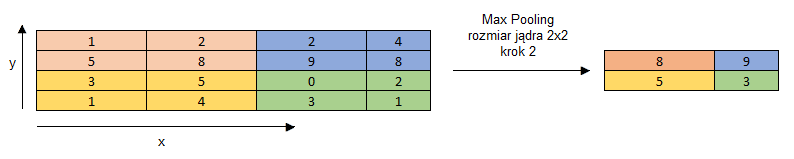
\includegraphics[width=17cm, height=4.5cm]{image//maxPoolingImg.png}
				\caption
				[Max pooling]
				{Max pooling}
			\end{figure}
        
			Pooling jest również metodą regularyzacji sieci neuronowej, zapobiegający jej przeuczeniu. 
        
        \par Inną efektywną drogą regularyzacji sieci neuronowych również zapobiegającą zjawisku przeuczenia się sieci jest dropout. 
			Podczas treningu sieci zostają wykluczone, dezaktywowane nadmiarowe neurony z architektury sieci w sposób losowy, 
			w efekcie może on uwzględniać np. neurony o najmniejszych wagach, które nie mają wiekszego wpływu na ostateczny wynik działania sieci. 
			Tak odrzucone neurony nie biorą już udziału w końcowym procesie wnioskowania. Obok dropout'u istnieją takie metody zapobiegające 
			przeuczeniu się sieci jak: legularyzacja l1 i l2, zmniejszające wartość absolutną, pierwiastek kwadratowy wag, uznając, że modele mające 
			zminimalizowane wagi osiągają lepsze wyniki. Legularyzacja, a w szczególności dropout pozytywnie wpływa na minimalizację błędu 
			klasyfikacji sieci neuronowej \textbf{dodanie przypisu i adresu strony lub przeklejenie wykresu z podaniem zrodla \href{https://leonardoaraujosantos.gitbooks.io//artificial-inteligence//content//dropout_layer.html}{\url{https://leonardoaraujosantos.gitbooks.io//artificial-inteligence//content//dropout_layer.html}}.
        }. 
        
			Kolejnym algorytmem powszechnie stosowanym w celu optymalizacji sieci neuronowych (wielowarstwowych) jest algorytm wstecznej propagacji błędów 
			\textit{(ang. backpropagation)}. Wagi poszczególnych połączeń mogą zostać wytrenowane, a więc dobrane automatycznie i stanowiące 
			w przybliżeniu zestaw najbardziej optymalny. Wsteczna propagacja błędów polega na aktualizowaniu wartości wag na podstawie wartości błędu 
			wag dotychczasowych. W celu poprawy efektywności wstecznej propagacji błędów często zaleca się następujące metody: 
			zastosowanie losowych wag początkowych, kilkukrotne powtarzanie procesu uczenia. Sam algorytm uwzględnia następujące kroki 
			zakładając losową generację wag początkowych: obliczenie odpowiedź sieci dla każdego z wektorów uczących, 
			każdy z neuronów wyjściowy oblicza swój błąd, propagacja błędów do warstw wcześniejszych, na podstawie propagowanej wartości 
			błędu każdy z neuronów modyfikuje wagi, powyższe kroki są powtarzane dopóki średni błąd nie przestanie maleć.

        \par Do budowy konwolucyjnych sieci neuronowych został wykorzystany framework Deeplearning4j. Działa on na wirtualnej maszynie Javy. 
			Można go wykorzystywać z językiem programowania Java (DL4J) i Scala (DL4S). Narzędzie posiada bogatą dokumentacje, repozytorium kodu na 
			platformie GitHub gdzie znajdują się zaimplementowane gotowe przykłady użycia frameworku 
			\href{https://github.com//deeplearning4j//nd4j}{\url{https://github.com//deeplearning4j//nd4j}}. Umożliwia konfigurację środowiska 
			za pośrednictwem narzędzi automatyzujących budowę projektu, na przykład: Maven, Gradle, Ivy, SBT. Do operacji backendowych narzędzie 
			udostępnia wybór pomiędzy GPU, a CPU. Framework posiada zaimplementowane mechanizmy budowy, regularyzacji, optymalizacji sieci neuronowych, 
			różnorodne rodzaje warstw z których możemy budować architekturę sieci (główne grupy) : Feed---Forward Layers, Output Layers, Convolutional Layers, 
			Recurrent Layers,  Unsupervised Layers, Other Layers, Graph Vertices, InputPreProcessors. 
			W pracy wykorzystywane są następujące z udostępnionych warstw wraz z konfiguracją: 

			\begin{spacing}{\spacingInSolemnItemize}
				\begin{itemize}
					\item ConvolutionLayer --- warstwa wykonująca konwolucję
						\begin{itemize}
							\item ConvolutionLayer.Builder (x, y) --- określa wielkość jądra; x --- jego szerokość w pikselach, a y --- jego wysokość w pikselach,
							\item stride (m, n) --- określa krok z jakim jądro jest przesuwane na obrazie wejściowym; m --- przesunięcie na osi odciętych w pikselach, 
								a n --- przesunięcie na osi odciętych w pikselach,
							\item nOut (k) --- określa liczbę filtrów przez które przechodzi obraz;
						\end{itemize}
					\item SubsamplingLayer --- warstwa odpowiadająca za pooling,
						\begin{itemize}
							\item SubsamplingLayer.Builder(SubsamplingLayer.PoolingType.n) --- n --- określa rodzaj poolingu z pośród: MAX, AVG, SUM, PNORM; 
							\item kernelSize (m, n) --- określa wielkość jądra; m --- jego szerokość w pikselach, a n --- jego wysokość w pikselach,
						\end{itemize}
					\item DenseLayer --- warstwa standardowa biorąca pod uwagę wszystkie wyjścia z warstwy poprzedniej \textbf{nie wiem jak to lepiej opisac},
					\item OutputLayer --- warstwa wyjściowa odpowiadająca za klasyfikację;
				\end{itemize}
			\end{spacing}
			
		\par Narzędzie wspiera następujące parametry konfiguracji sieci lub poszczególnych warstw: funkcja aktywacji, inicjalizacja wag początkowych, 
			aktualizacje kroku uczenia, regularyzację i inne.
			\newline
		
            \lstinputlisting[caption=Przykładowa konfiguracja konwolucyjnej sieci neuronowej]{przykladowaSiec.java}
		
        \par Wszystkie dostępne warstwy i parametry konfiguracji sieci dostępne są na stronie projektu:
			\href{https://deeplearning4j.org//quickref\#config}{\url{https://deeplearning4j.org//quickref\#config}}.
        
	\subsection{Tesseract OCR}
	    \paragraph{\indent} Tesseract jest systemem służącym do optycznego rozpoznawania znaków (OCR \textit{ang. optical character recognition}) 
			opracowanym przez firmę HP, obecnie projekt jest sponsorowany przez Google. System został napisany w języku C. 
			Dostępne są interfejsy umożliwiające korzystanie z narzędzia, z poziomu innych języków np. Java (wrapper Tess4J). 
			\par Pierwsza wersja umożliwiała pracę z językiem angielskim, kolejne wydania powiększały listę pakietów językowych, 
			najpierw o inne języki zachodnioeuropejskie, a później o inne języki. Na szczególna uwagę wśród nich zasługują japoński, chiński, 
			i języki semickie czytane od prawej do lewej. Obecne narzędzie udostępnia wybór pakietu językowego uwzględniającego 
			znaki diakrytyczne wśród około 130 możliwych. Oprócz obsługi różnych języków możliwa jest obsługa różnych czcionek. 
			\par W początkowej wersji Tesseract pozwalał na pracę z plikami o rozszerzeniu TIFF. Kolejne wersje systemu umożliwiają pracę z bogatszą gamą plików: 
			JPEG, GIF, PNG, BMP, wielostronicowych plików TIFF dzięki wykorzystaniu biblioteki służącej do przetwarzania obrazów --- Leptonica 
			(wrapper Java --- Lept4J). Dzięki współpracy dodatkowych bibliotek (GPL Ghostscript lub PDFBox) możemy odczytywać tekst zawarty w plikach PDF. 
			\par Dodatkowymi funkcjonalnościami, które zasługują na uwagę są: możliwość analizy układu strony, uzyskania informacji o położeniu rozpoznanego tekstu na stronie 
			i formatowanie tekstu wyjściowego. 
			\par Projekt dostępny jest na wielu platformach: Windows, Linux, Mac OS X. Tesseract nie udostępnia graficznego interfejsu użytkownika, 
			a sama konfiguracja systemu i przetwarzanie danych odbywa się z poziomu konsoli, powstały jednak systemy wykorzystujące tesseracta i posiadające GUI. 
			\par Oprogramowanie w pewnych okolicznościach jest wrażliwe na błędy, należy unikać rozmiaru tekstu mniejszego niż 20px, pochylonego lub obróconego, 
			niepozytywnie na działanie wpływają również ciemne granice strony ponieważ mogą one zostać rozpoznane i dopasowane jako znaki.
	    \par Silnik tesseracta uznawany jest za jeden z najlepiej działających wśród dostępnych systemów OCR. 

	\subsection{Środowisko programistyczne}
		\paragraph{\indent} Projekt powstał w technologii Java. Utrzymująca się popularność tej technologii na pierwszym miejscu 
			(która wciąż rośnie)\footnote{\href{https://www.tiobe.com//tiobe-index}{\url{https://www.tiobe.com//tiobe-index}}, dostęp 2018.07.22} 
			wśród języków programowania ułatwi dalszy rozwój i wsparcie aplikacji. 
		
		\par W wersji 8, wprowadzone zostały znaczące kamienie milowe takie jak: wyrażenia lambda oraz strumienie. Zostały one wykorzystane 
			w kodzie źródłowym aplikacji, przez co znacząco przyśpieszyły działanie, wykonywanie poszczególnych metod i podniosły czytelność, zwięzłość kodu. 
        
		\par Wykorzystanym IDE \textit{(ang. integrated development environment)} było Eclipse. Po utworzeniu projektu Maven, do pliku pom.xml 
			dodano zależności umożliwiające wykorzystanie funkcjonalności Tesseract oraz zależności umożliwiające pracę z frameworkiem DL4J. 
			Ponadto do projektu została dołączona biblioteka OpenCv jako biblioteka użytkownika. Wykorzystanie technologii Maven 
			w znaczący sposób ułatwiło zarządzanie zależnościami i wykorzystanymi bibliotekami w projekcie.
        \newpage
        
\section{Część praktyczna}
	\subsection{Budowa aplikacji}
		\paragraph{\indent} Algorytmy  przetwarzające obrazy zostały umieszczone w odpowiednich klasach, ułatwiających posługiwanie się nimi. Rozwiązanie to wychodzi na przeciw podstawowym zasadą obiektowości takimi jak: modularyzacja, hermentyzacja, abstrakcja. W aplikacji można wyróżnić następujące funkcjonalności i odpowiadające im klasy:
		\begin{spacing}{\spacingInSolemnItemize}
    		\begin{enumerate}
    			\item ekstrakcja stron z pliku pdf do obrazów (jedna strona pliku pdf odpowiada jednemu obrazowi) --- klasa GetImgFromPdf;
    			\item polepszenie jakości obrazu --- klasa ImproveImg;
    			\item usunięcie z obrazu obszarów które nie należą do stron --- klasa CutBlackArea;
    			\item podział obrazu na dwie strony --- klasa DivideToPage;
    			\item przygotowanie obrazu do analizy poprzez budowę zbiorów linii --- klasa PrepareImgToAnalize;
    			\item wyprostowanie obrazu --- klasa ToStraightenUp;
    			\item zasadnicze przetwarzanie obrazu, detekcja obszarów zawierających znaki muzyczne i teksty --- klasa MajorProcessing; 
    			\item wykrycie tekstu --- klasa DetectText;
    			\item rozpoznanie oraz wycięcie konturów obrazu które tworzą litery, znaki interpunkcyjne, etc. --- klasa DetectLetter;
    			\item  model, konfiguracja, uczenie się konwolucyjnych sieci neuronowych, odpowiednio klasyfikującej litery, linie czy jest linią tekstu czy nut --- klasa LetterClassifier i klasa MusicSheetClassifier;
    			\item wykorzystanie zserializowanych konwolucyjnych sieci neuronowych w celu przetworzenia danych wejściowych i zwróceniu wyniku, odpowiednio tekstu, wartości logicznej --- klasa ReadLetterClassifier i klasa MusicSheetClassifierImg;
    		\end{enumerate} 
        \end{spacing}
    
        \par Powyższe funkcjonalności systemu zostały dokładniej opisane w kolejnych podrozdziałach.

	\subsubsection{Ekstrakcja stron z plików pdf}
		\paragraph{\indent} Przy pomocy biblioteki Apache PDFBox dołączonej do projektu jako plik z rozszerzeniem jar, z plików pdf można pobrać strony konwertując je do kolorowych plików graficznych z określoną rozdzielczością. Metody które wykonują powyższe algorytmy zawarte są w klasie GetImgFromPdf.

        %\newpage
        
		\begin{figure}[!ht]  
			\begin{center}
				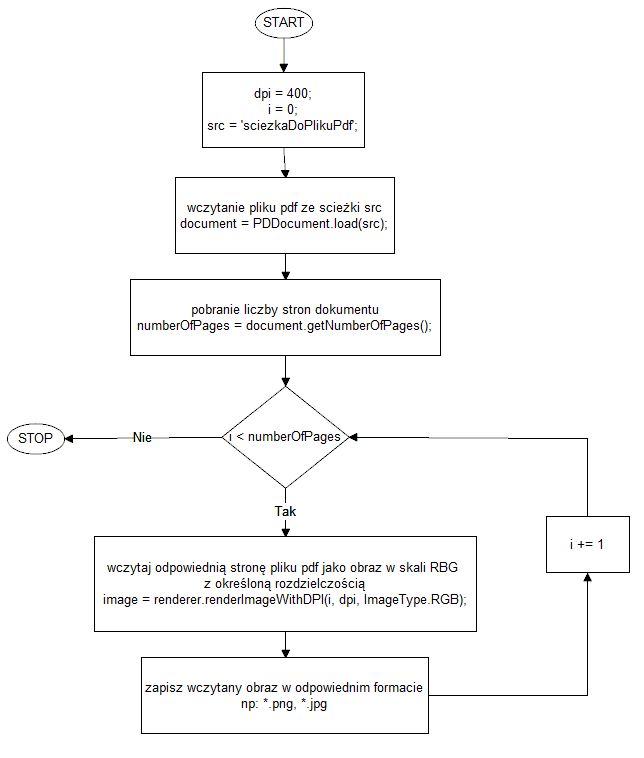
\includegraphics[height=19cm]{image//algorithm//getImgFromPdf.png}%[width=15cm, height=18cm] {image//algorithm//getImgFromPdf.png} 
			\end{center}
			\caption
    			[Algorytm pobierania obrazów z plików pdf]  
	    		{Algorytm pobierania obrazów z plików pdf}  
		\end{figure}
		\newpage
		\subsubsection{Polepszenie jakości obrazów}
			\paragraph{\indent} Algorytmy polepszające jakość obrazu zostały zaimplementowane w klasie           ImproveImg. Redukują szumy, dzięki wykorzystaniu metod rozmycia i        progowania udostępnionych przez bibliotekę OpenCv, które pracują na         obrazie wczytanym w skali szarości.  
			\par
			    Operacja rozmycia nosi również nazwę wygładzania, przyczyny wykonania zabiegu rozmycia na obrazie mogą być różne, w znaczącej większości przypadków powodem jest chęć usunięcia występujących szumów. Do wyboru (w bibliotece OpenCv) mamy kilka funkcji, posługujących się różnymi rodzajami filtrów dolnoprzepustowych, a więc wykorzystującymi różne jądra, będące de facto współczynnikami tych filtrów. Algorytm wykorzystuje funkcję:
			    \textit{Imgproc.medianBlur (src, dst, ksize);}
			    gdzie \textit{ksize} jest rozmiarem jądra, które jest nieliniowe oraz:  
			    
			    \begin{displaymath}
                    ksize\, \epsilon\, \mathbb{N}\, \wedge\, ksize\, \epsilon\, \mathbb{Z}\, \wedge\, ksize\pmod{2} = 1
                \end{displaymath}
                
                \par Filtr ten wartości poszczególnych pikseli zmienia na medianę, która zostaje obliczona uwzględniając wartości pikseli tworzących określony prostokąt w którego centrum jest zmieniany piksel. 
                
                \par
			    Jedną z najprostszych metod segmentacji obrazu jest operacja progowania.  Biblioteka udostępnia dwa warianty progowań: proste i adaptacyjne. 
			    Wśród progowań prostych możemy wybrać jedną z następujących możliwości  \textit{(thresholdType)}: BINARY, BINARY\_INV, TRUNC, TOZERO, TOZERO\_INV.
			    Algorytm wykorzystuje proste progowanie binarne (BINARY), które wartość każdego z pikseli obrazu \textit{(src)} porównuje z zadanym progiem \textit{(threshold)} i jeśli jego wartość jest od niego większa to, temu pikselowi przypisywana jest wartość \textit{maxValue}, następnie obraz zapisywany jest w nowej macierzy \textit{(dst)}.\\
			    \textit{Imgproc.threshold (src, dst, threshold, maxValue, thresholdType//*Imgproc.THRESH\_BINARY*//);}
			    
			    \begin{displaymath}
                    dst (x, y) =  
                    \left\{
                        \begin{array}{ll}
                            maxValue & \textrm{dla } src (x, y) > threshold \\
                            0 & \textrm{dla } src (x, y) \leqslant threshold
                        \end{array}
                    \right.
                \end{displaymath}
			    
			    \newpage
    		    
    		    \begin{figure}[!ht]  
    			    \begin{center}
    			        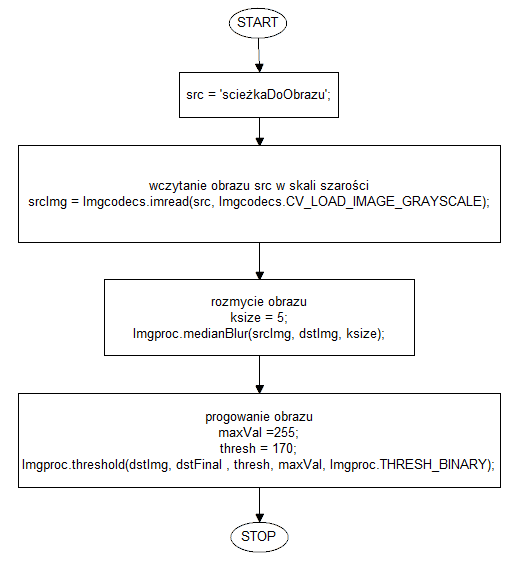
\includegraphics[]{image//algorithm//improveImg.png}%[width=12cm, height=12cm] {image//algorithm//improveImg.png} 
    			    \end{center}
    			    \caption
        			    [Algorytm polepszenia jakości obrazów]  
	    		        {Algorytm polepszenia jakości obrazów}  
    		    \end{figure}
		
                \newpage
		
    		    \begin{figure}[!ht]  
    			    \begin{center}
    				    \includegraphics[height=10.5cm, frame] {image//exampleImage//001_a.jpg} 
    			    \end{center}
    			    \caption
        			    [Obraz przed zastosoawaniem algorytmu]  
                        {Obraz przed zastosoawaniem algorytmu}  
    		    \end{figure}
		
		        \begin{figure}[!ht]  
    			    \begin{center}
    				    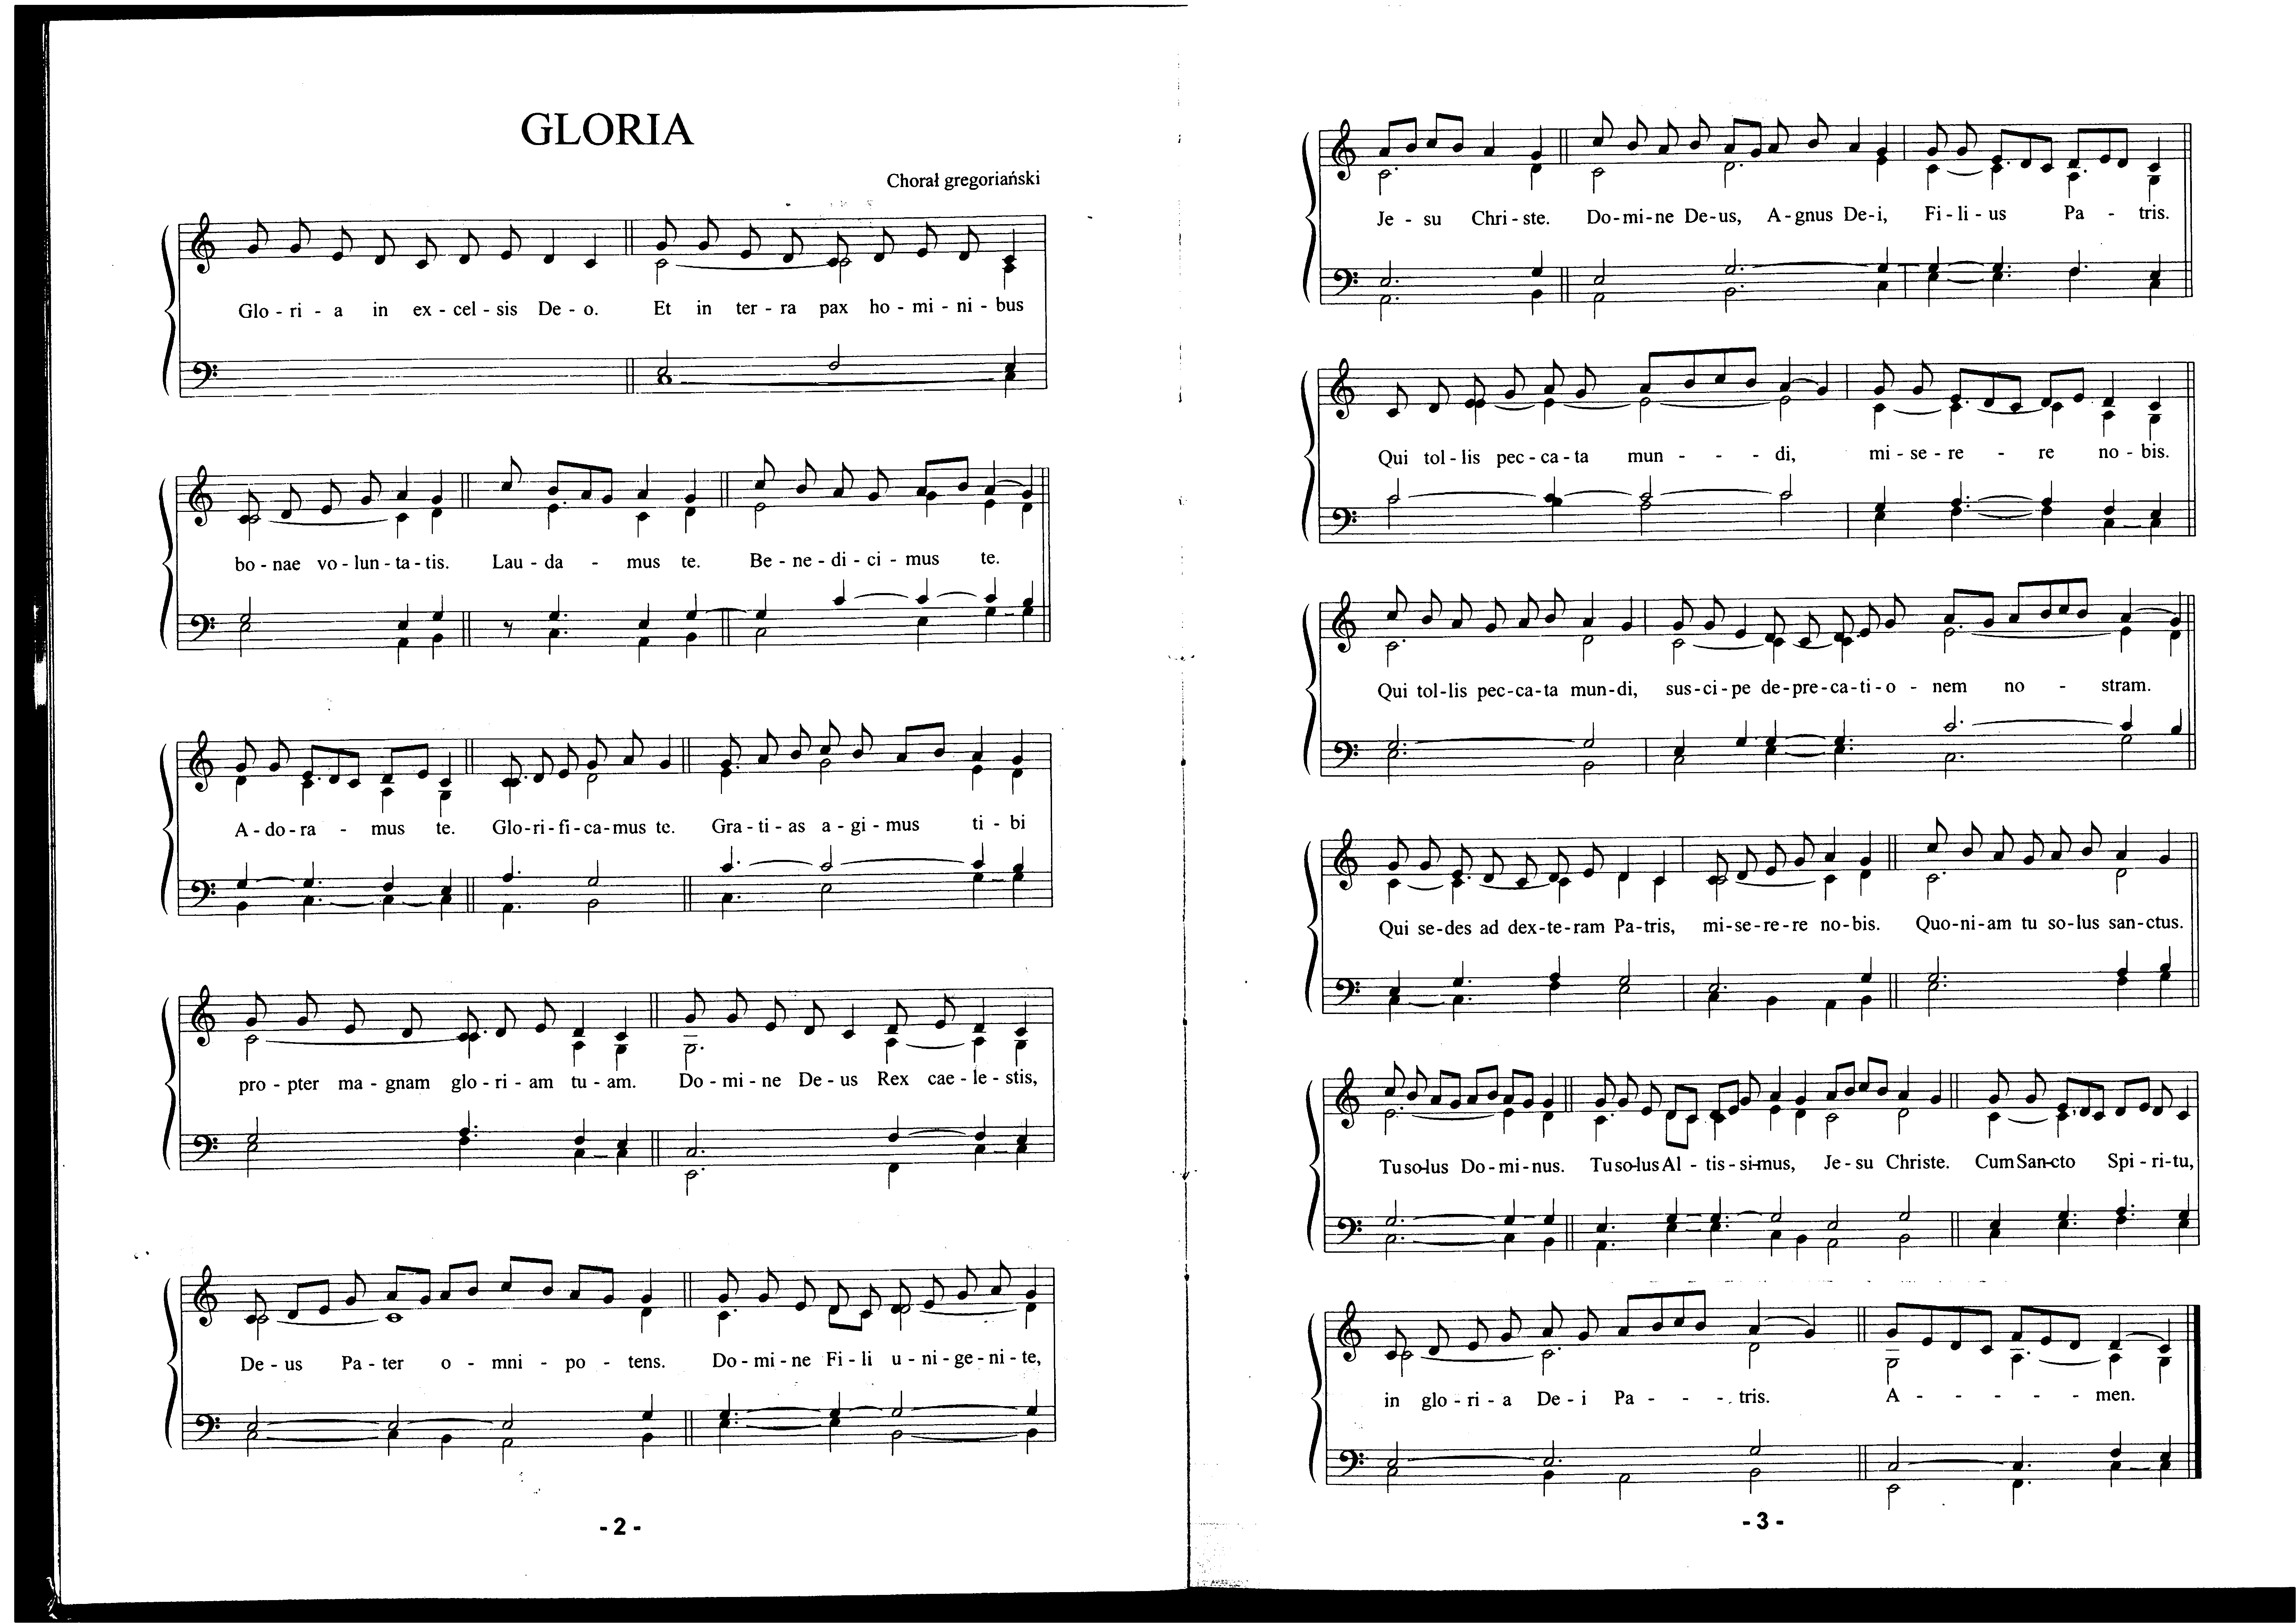
\includegraphics[height=10.5cm, frame] {image//exampleImage//001_b.png} 
    			    \end{center}
	    		    \caption
    			        [Obraz po zastosowaniu algorytmu]  
	    		        {Obraz po zastosowaniu algorytmu}  
	            \end{figure}
		
		\subsubsection{Eliminacja nadmiarowych (czarnych) obszarów skanu}
			\paragraph{\indent} 
			Algorytm wykrywający i usuwający czarne obszary skanu (uzupełnienie skanu do określonego formatu np. A4) zostały  zaimplementowane w klasie CutBlackArea. Algorytm wykorzystuje do tego           wartości odchylenia standardowego w poziomych liniach obrazu i wartości     dominanty. Przy założeniu, że powierzchnie te znajdują się po lewej         stronie i na dole obrazu. Algorytm umożliwia wycięcie jednego (dolnego)     lub obu obszarów. 
			
    			\begin{figure}[!ht]  
    			    \begin{center}
    				    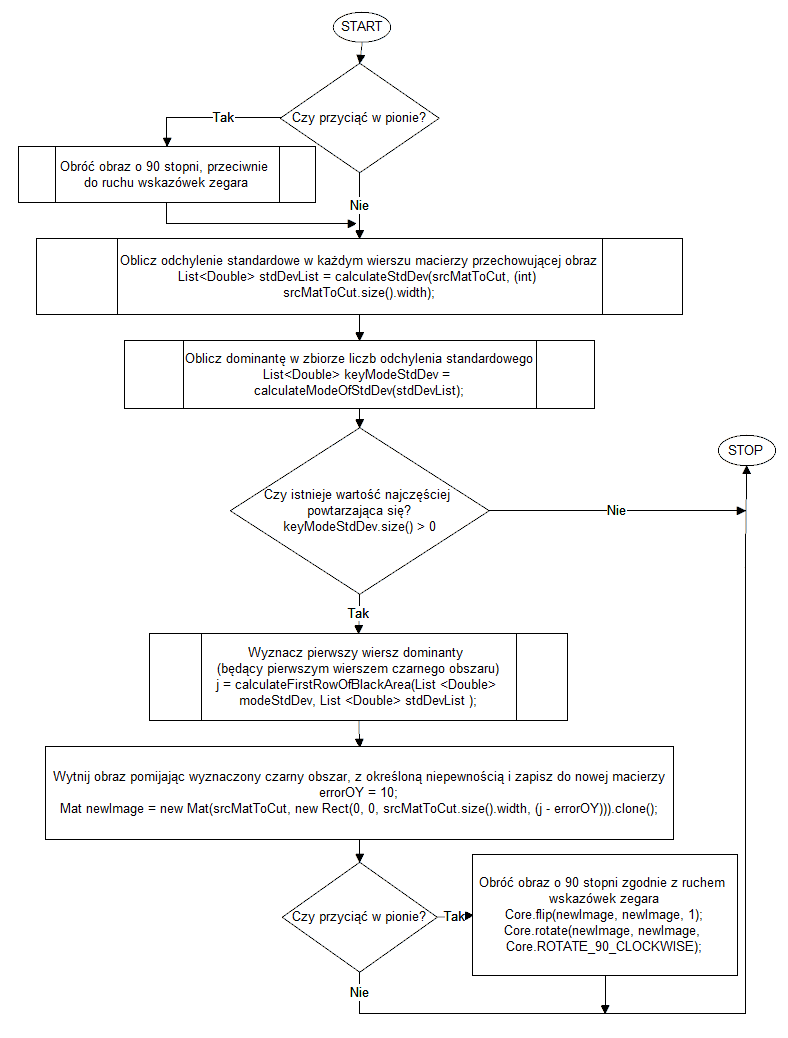
\includegraphics[height=18cm] {image//algorithm//cutBlackArea.png} 
    			    \end{center}
    			    \caption
        			[Algorytm usuwający czane obszary z obrazu]  
    	    		{Algorytm usuwający czane obszary z obrazu}  
    		    \end{figure}
		    
		        \newpage
		    
    		    \begin{figure}[!ht]  
    			    \begin{center}
    				    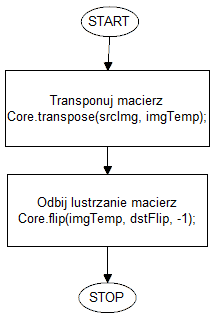
\includegraphics[] {image//algorithm//cutBlackAreaPredv2.png} 
    			    \end{center}
    			    \caption
            			[Poszczególne funkcje algorytmu a) Obrót o 90 stopni zgodnie z ruchem wskazówek zegara]  
        	    		{Poszczególne funkcje algorytmu a) Obrót o 90 stopni zgodnie z ruchem wskazówek zegara}
    		    \end{figure}
			    
			    %\guilsinglleft
			
		        \lstinputlisting[caption=Metoda obliczająca odchylenie standardowe każdej linii]{calculateStdDev.java}
		        \newpage
		        
			    \lstinputlisting[caption=Metoda obliczająca początek czarnego obszaru]{calculateFirstRowOfBlackArea.java}
	        
    			\begin{figure}[!ht]  
    			    \begin{center}
    				    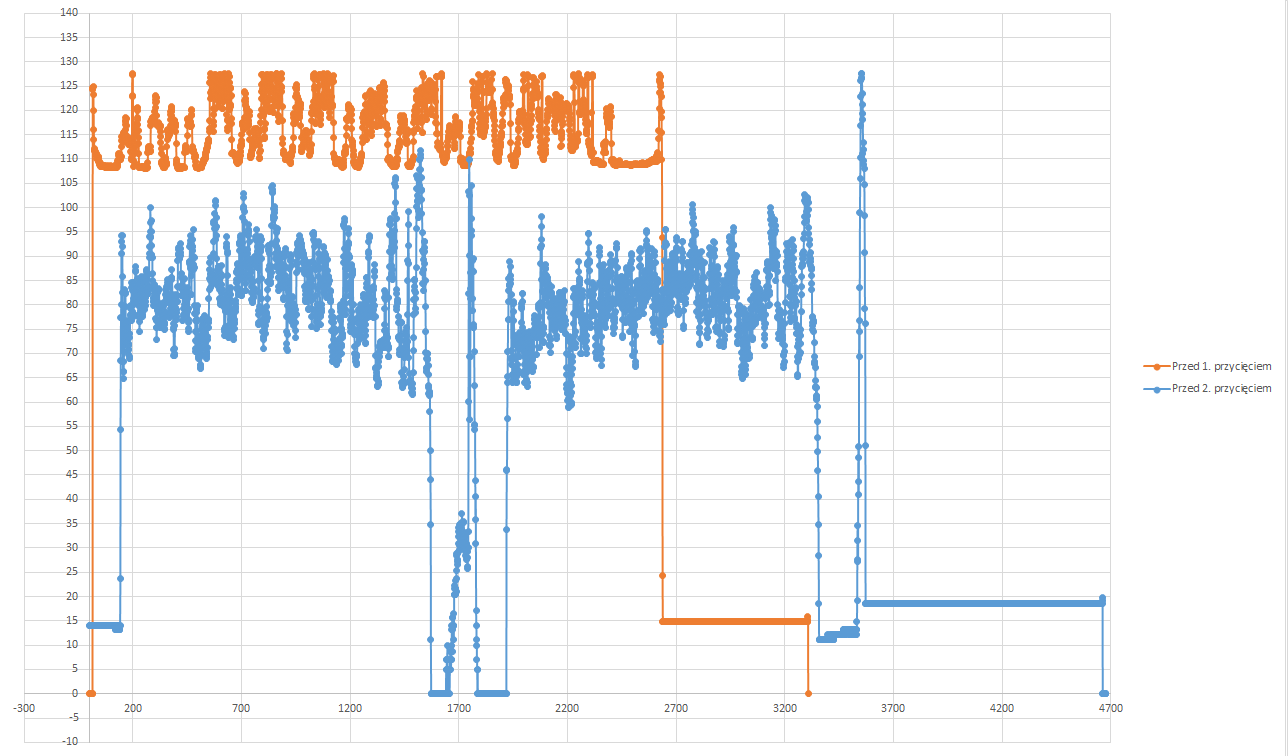
\includegraphics[height=10.5cm, frame] {image//practicalPart//stdDevCutBlackArea.png} 
    			    \end{center}
    			    \caption
            			[Odchylenie standardowe w funkcji wieszy macierzy] 
            			{Odchylenie standardowe w funkcji wieszy macierzy}  
    		    \end{figure}
			
    			Na podstawie wykresu można zauważyć, że wiersze obrazu (w skali szarości) o małej zmienności wartości pikseli, będą dawały niewielkie wartości odchylenia standardowego. Jeśli nie równa się ono zeru, ale jest odpowiednio małe można założyć, że badany wiersz ma jedną barwę, a wartość ta wynika z drobnych zakłóceń i niedoskonałości obrazu.
    			
    			Do obliczenia odchylenia standardowego została użyta funkcja udostępniona w bibliotece OpenCv:\textit {Core.meanStdDev(Mat src, MatOfDouble mean, MatOfDouble stddev)}. Oblicza ona średnią i odchylenie standardowe macierzy podanej jako parametr src (w algorytmie jest to jeden wiersz obrazu), które zależy od wszystkich kanałów macierzy. Tutaj jest to jeden kanał --- obraz przed obliczeniami został przetransformowany do skali szarości według poniższego algorytmu:
    			 		
			    \lstinputlisting[caption=Metoda transformująca obraz barwny do skali szarości]{toGrayScale.java}		
    			 		
    			Za obliczenie wartości najczęściej występującej odchylenia standardowego odpowiada funkcja: \textit {public List \guilsinglleft Double\guilsinglright calculateModeOfStdDev(List \guilsinglleft Double\guilsinglright stdDevList)}
    			wykorzystująca nowe rozwiązania wprowadzone w Javie wersji 8, a więc strumienie i wyrażenia lambda, co znacząco przyśpiesza czas obliczeń oraz przejrzystość napisanego kodu. 
    			\newline
			
			    \lstinputlisting[caption=Metoda obliczająca dominante odychylenia standardowego]{calculateModeOfStdDev.java}
			
    		    \begin{figure}[!ht]  
    			    \begin{center}
    				    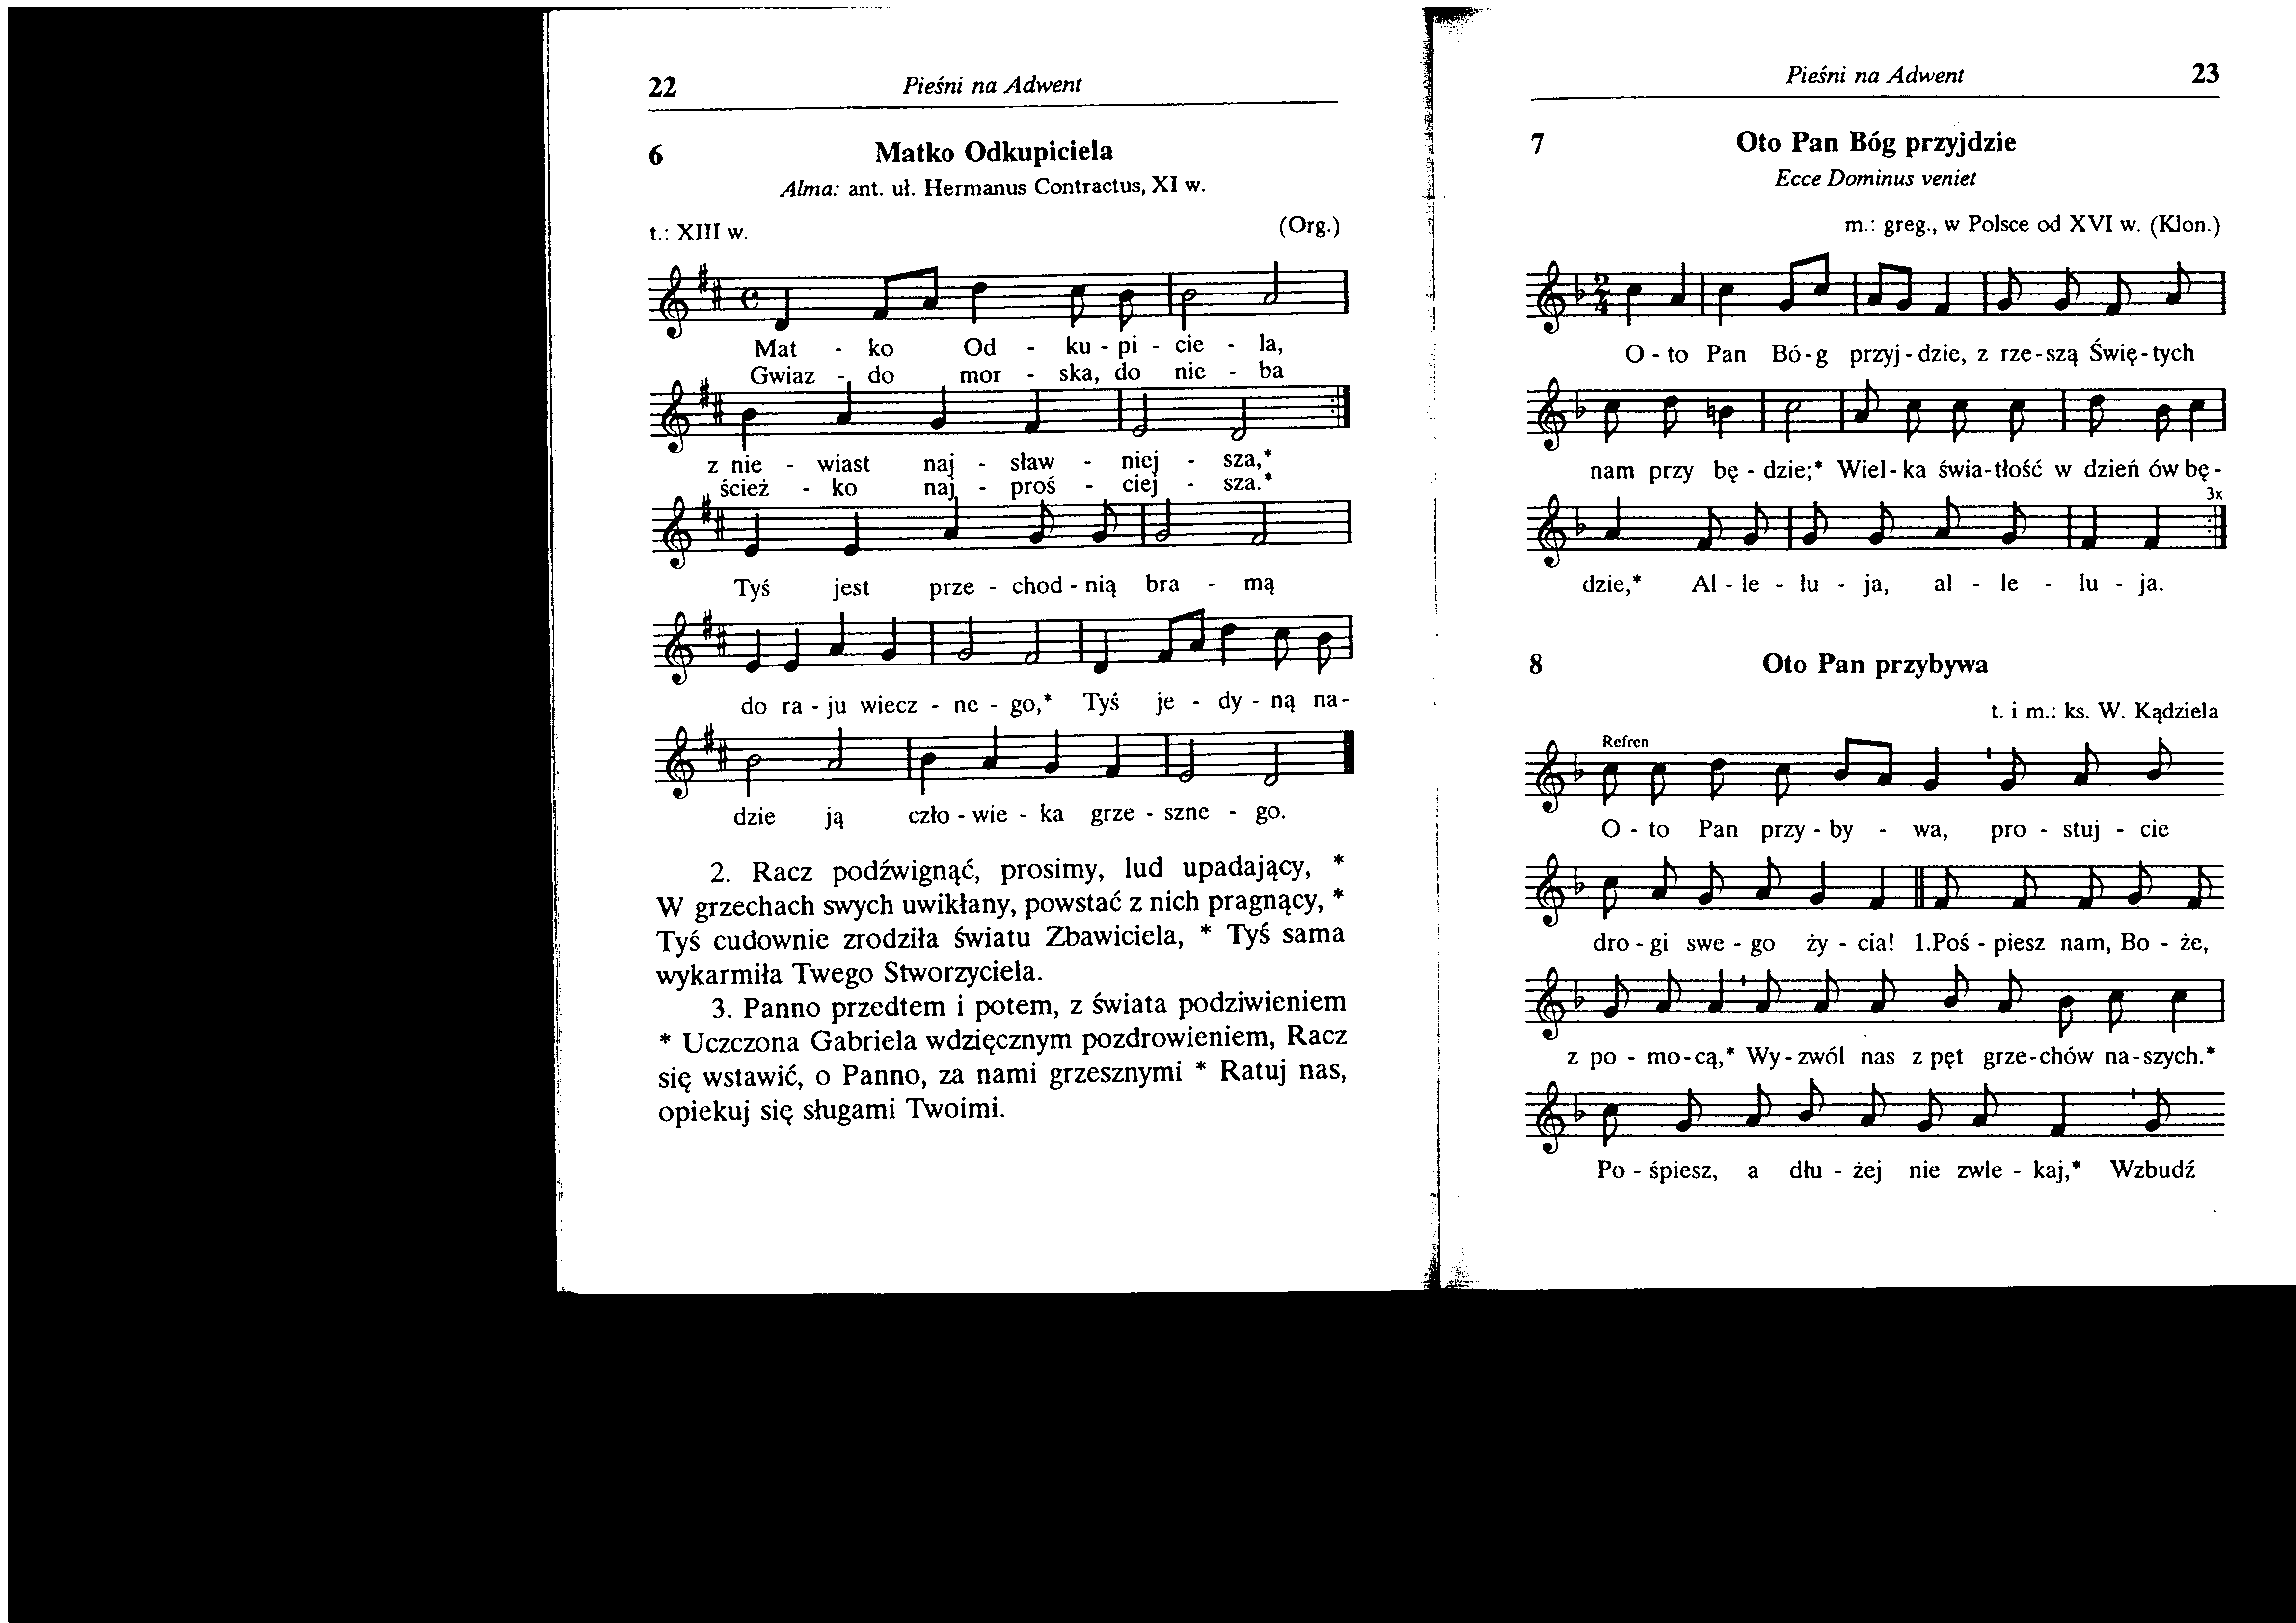
\includegraphics[height=11cm, frame] {image//exampleImage//002_a.png} 
    			    \end{center}
    			    \caption
    			        [Obraz przed usunięciem nadmiarowych obszarów]
        			    {Obraz przed usunięciem nadmiarowych obszarów}  
    		    \end{figure}
    		    
    		    \begin{figure}[!ht]  
    			    \begin{center}
    				    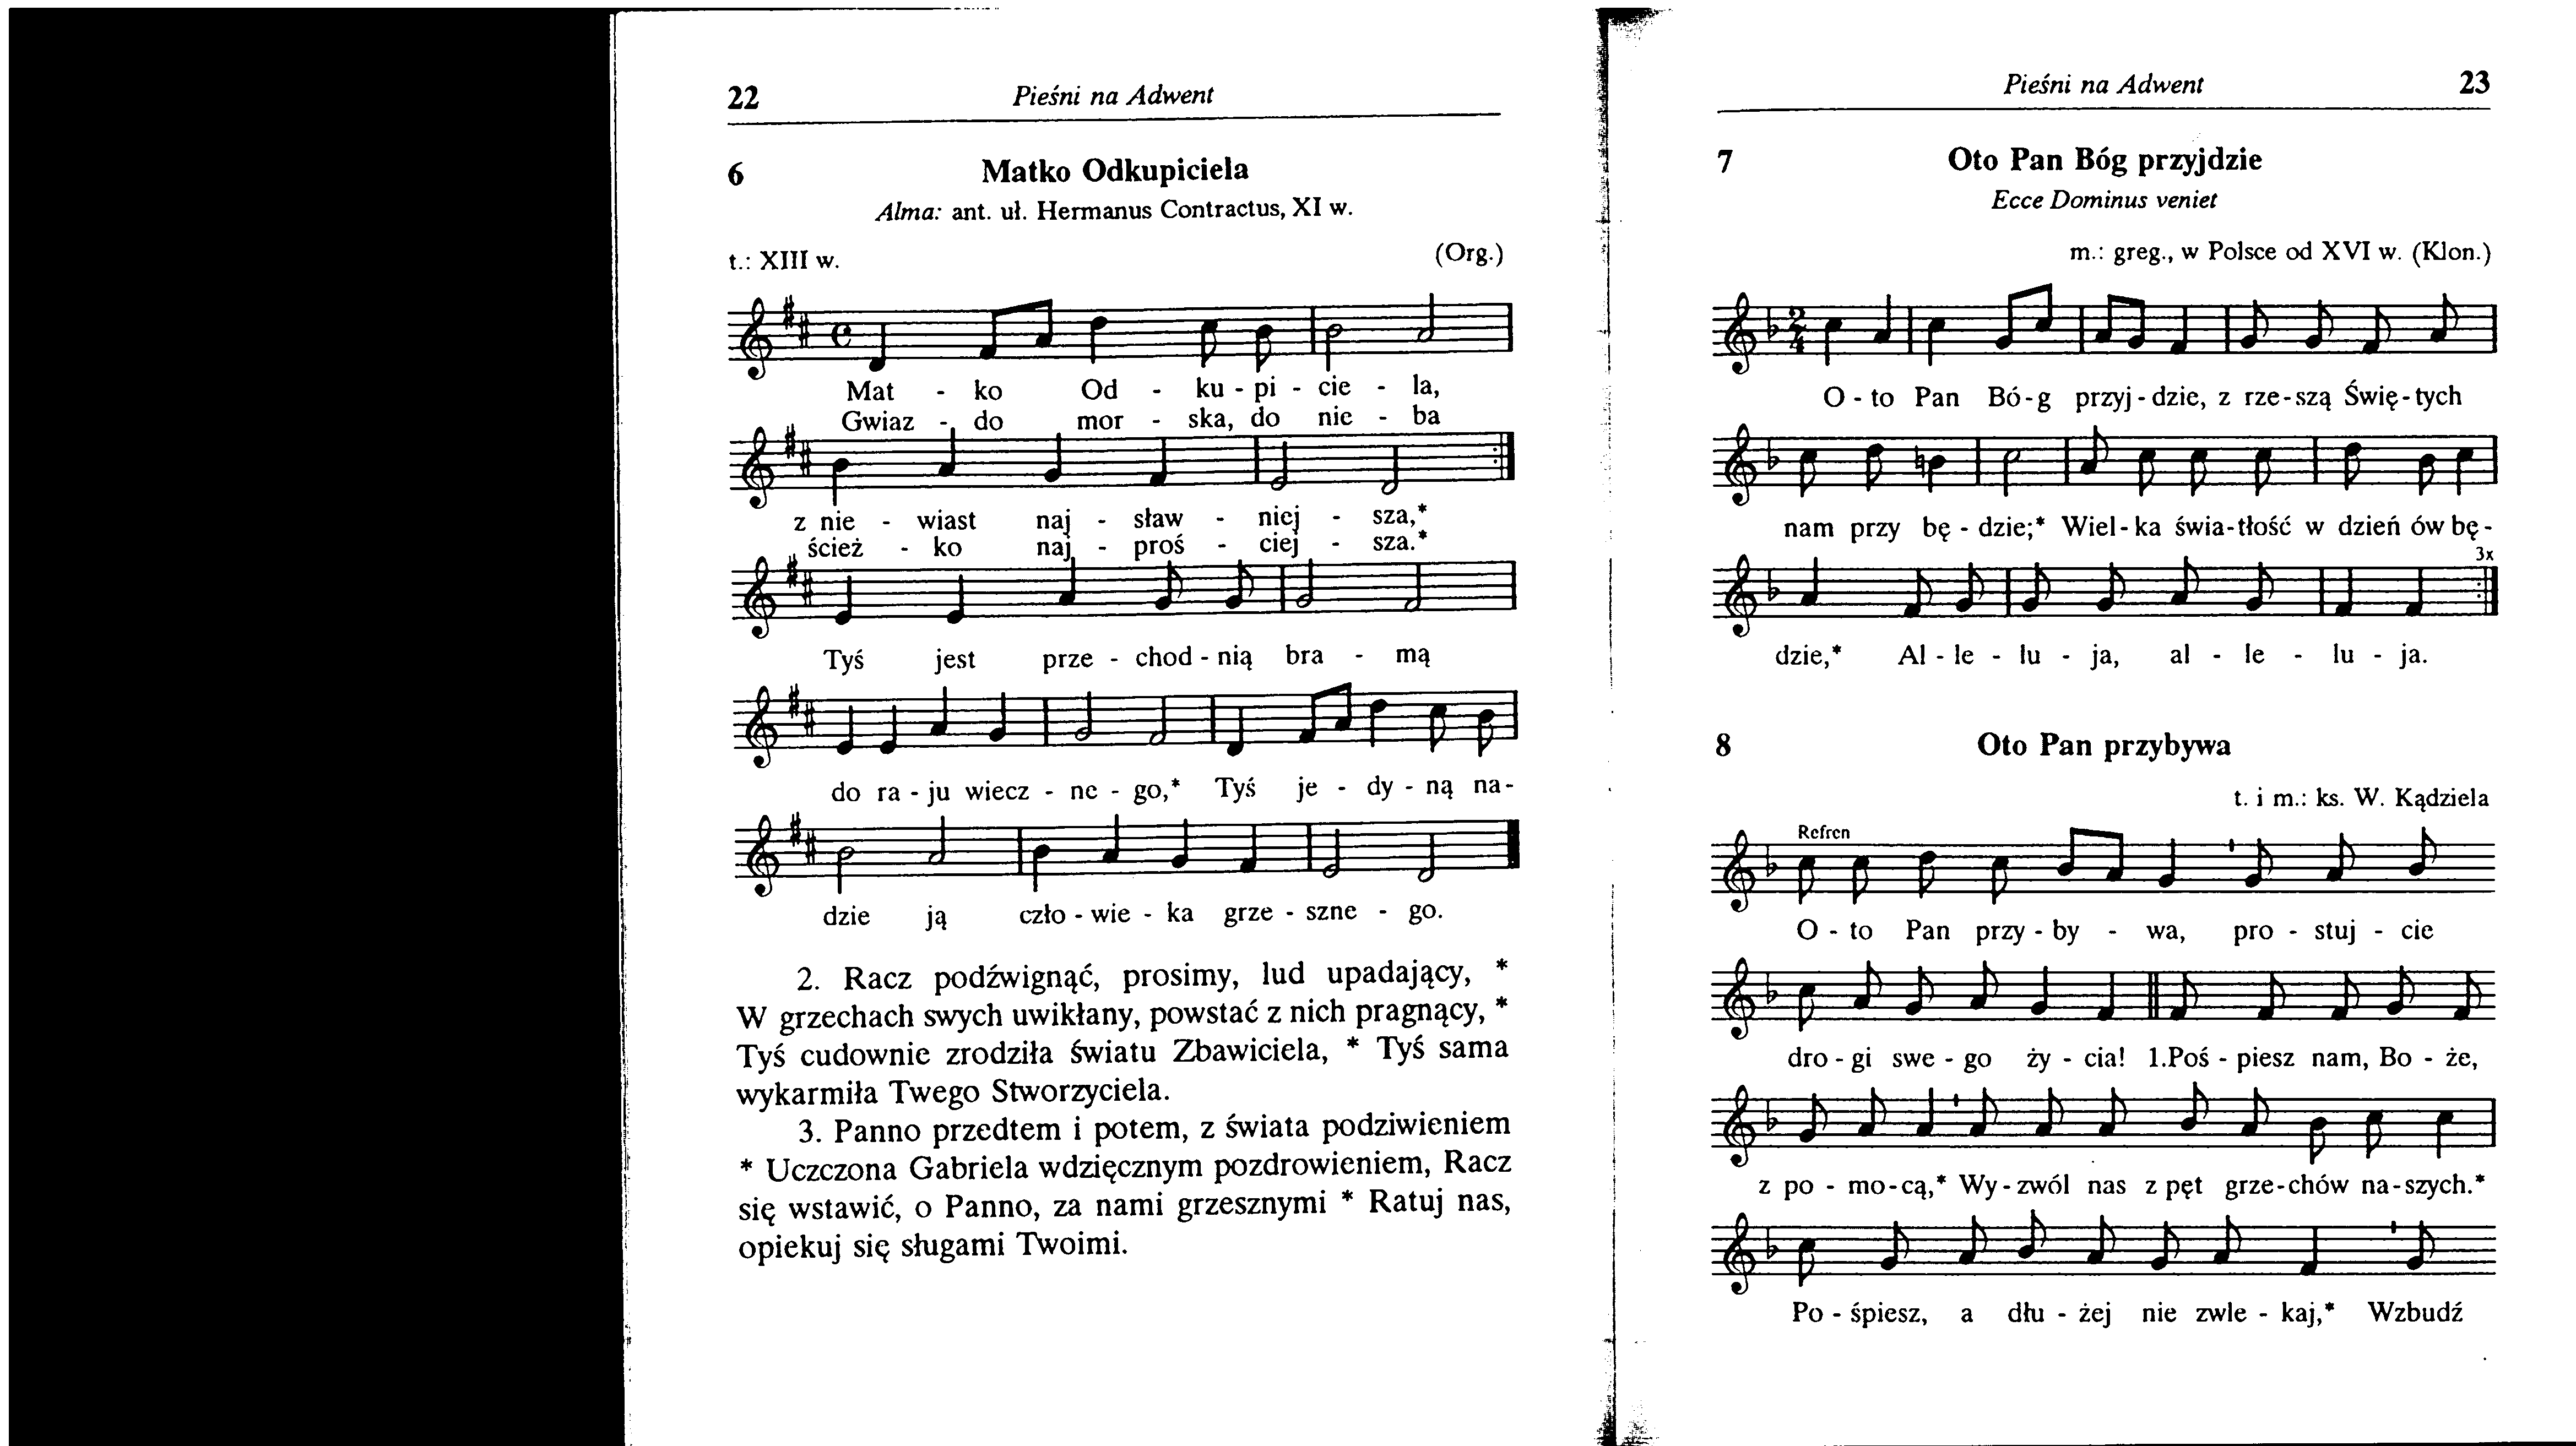
\includegraphics[height=10cm, frame]{image//exampleImage//002_b.png} 
    			    \end{center}
    			    \caption
            			[Obraz po przycięciu obszaru znajdującego się na dole] 
        			    {Obraz po przycięciu obszaru znajdującego się na dole}  
    		    \end{figure}
    			
    	        \begin{figure}[!ht]  
    			    \begin{center}
    				    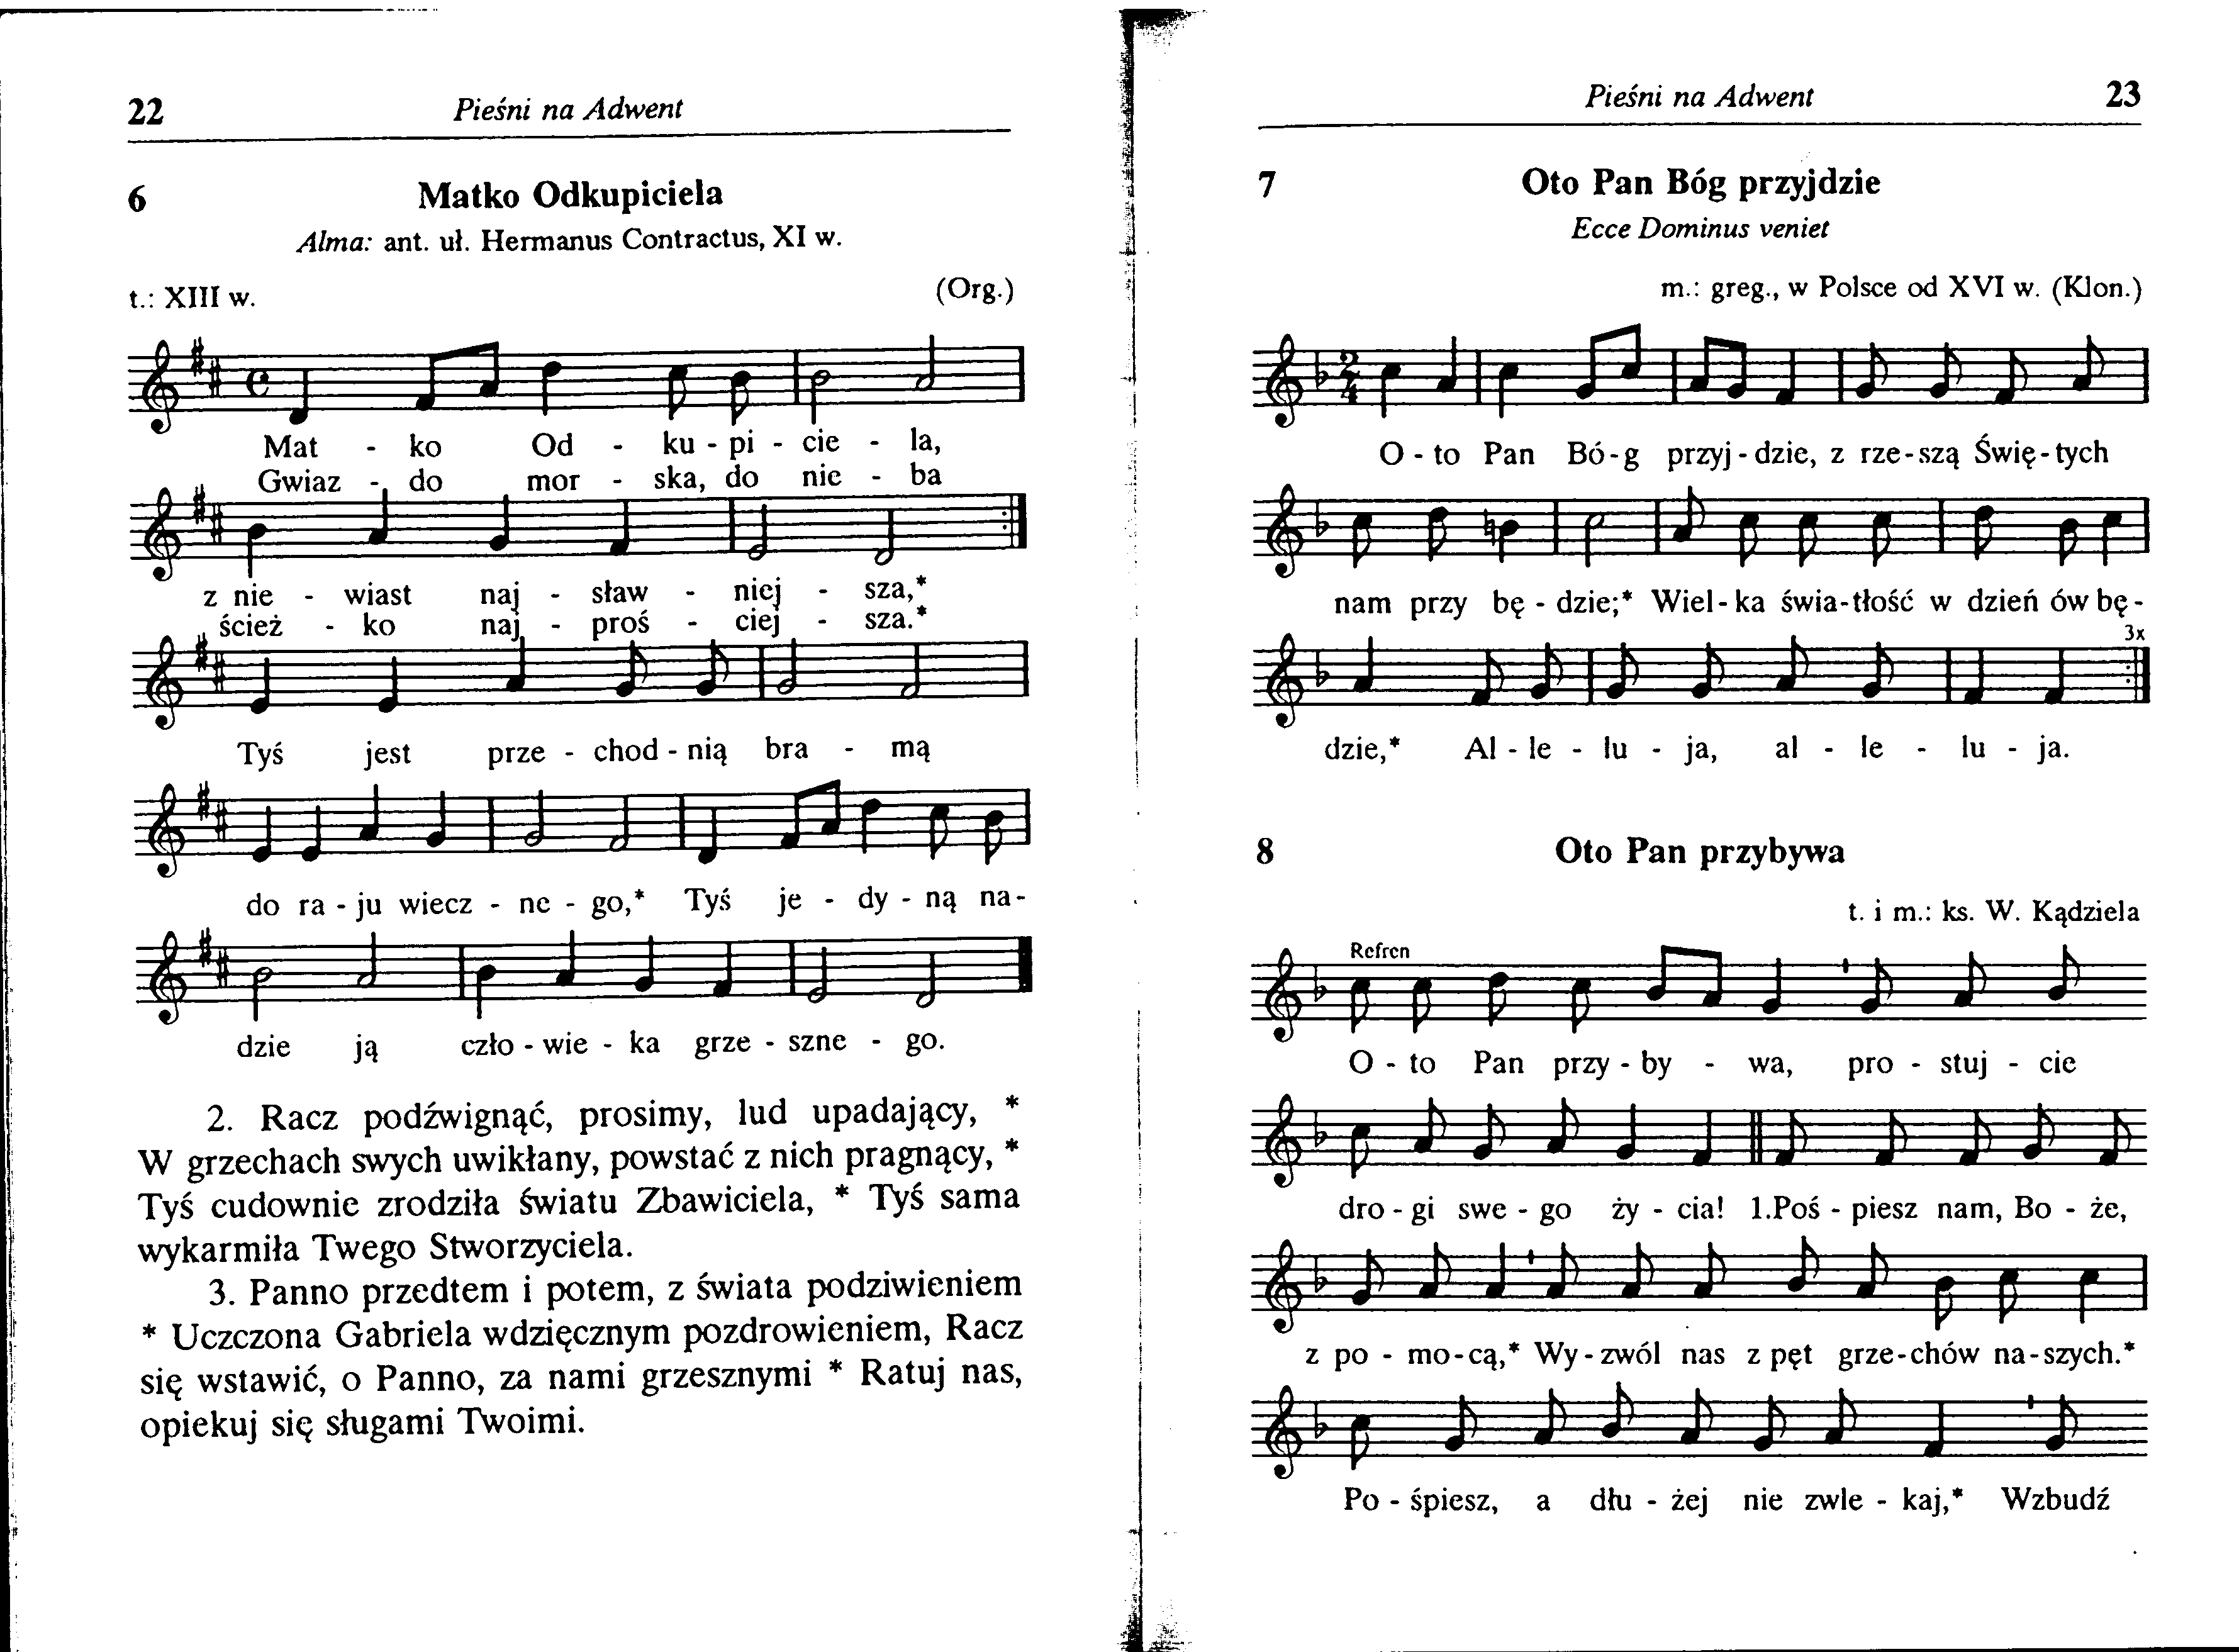
\includegraphics[height=12.5cm, frame] {image//exampleImage//002_c.png}
    			    \end{center}
        			\caption
        			    [Obraz po przycięciu obszaru znajdującego się po lewej stronie]
        			    {Obraz po przycięciu obszaru znajdującego się po lewej stronie} 
    		    \end{figure}

		\subsubsection{Podział skanu na dwie strony}
		    \paragraph{\indent} Algorytmy dzielące skan zawierającego dwie strony śpiewnika na dwa osobne obraz, z których każdy stanowi jedną stronę
		    zostały zaimplementowane w klasie DivideToPage. Algorytm wykorzystuje do tego niedoskonałość          skanu, który w książkach szczególnie tych o znacznej liczbie stron          odciska na ich łączeniu charakterystyczny czarny lub zaciemniony          obszar pionowy. Jeżeli wykrycie tego obszaru nie jest możliwe (niewielka    liczba przypadków) przyjęto założenie, że na cały obszar obrazu przypadają dwie strony śpiewnika i następnie zostaje on podzielony na dwie części gdzie granicą jest środkowa kolumna macierzy przechowującej obraz.    
		    
    	        \begin{figure}[!ht]  
    			    \begin{center}
    				  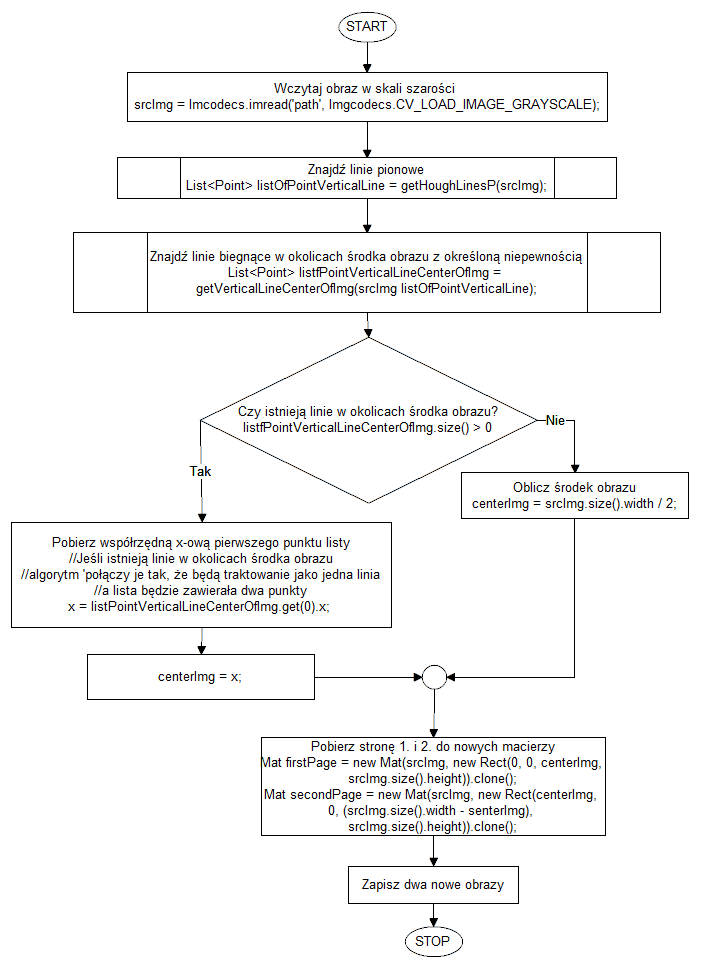
\includegraphics[height=22.5cm]{image//algorithm//divideToPage.png} 
    			    \end{center}
    			    \caption
        			    [Algorytm dzielący obraz na dwie części, strony]
        			    {Algorytm dzielący obraz na dwie części, strony}  
    		    \end{figure}
    		
    		\newpage
    		
    	        \begin{figure}[!ht]  
    			    \begin{center}
    				    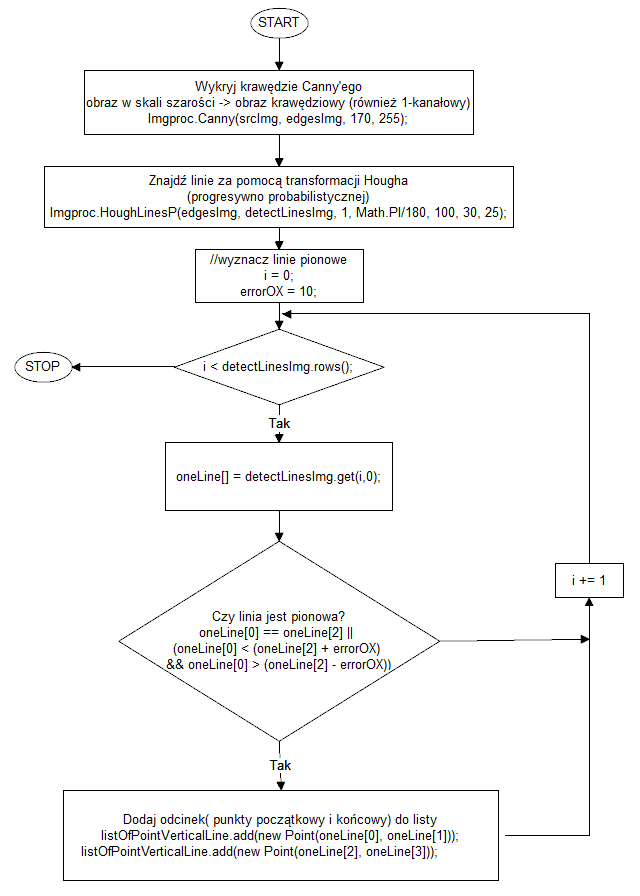
\includegraphics[height=22.5cm]{image//algorithm//divideToPagePred_01.png} 
    			    \end{center}
    			    \caption
        			    [Algorytm znajdujący linie pionowe]  
        			    {Algorytm znajdujący linie pionowe}  
    		    \end{figure}
		
    	        \begin{figure}[!ht]  
    			    \begin{center}
    				    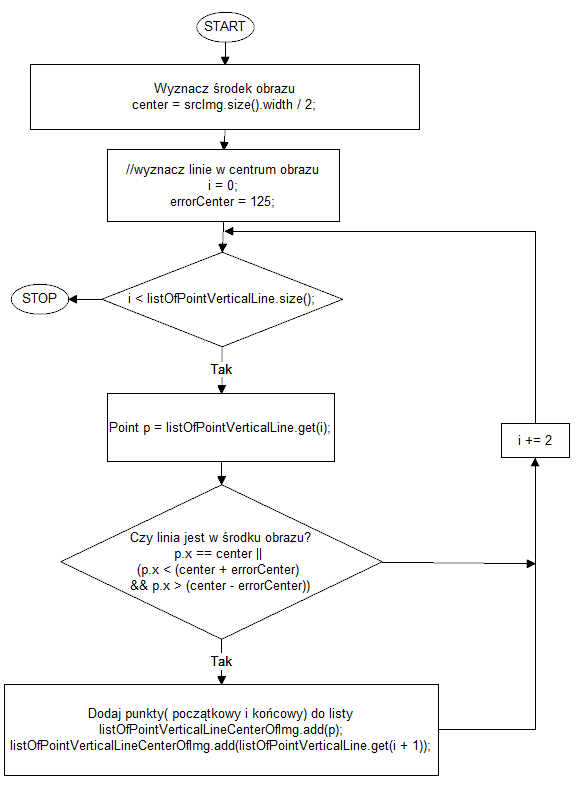
\includegraphics[height=22.5cm ]{image//algorithm//divideToPagePred_02.png} 
    			    \end{center}
    			    \caption
        			[Algorytm znajdujący linie pionowe w okolicach środka obrazu]  
        			{Algorytm znajdujący linie pionowe w okolicach środka obrazu}  
    		    \end{figure}
		
		        \newpage
		
		        Metoda ta korzysta z dwóch zasadniczych funkcji zaimplementowanych w bibliotece OpenCv - detektora krawędzi Canny'ego oraz transformacji (liniowej) Hougha. \par
		
		        %Detektor krawędzi Canny'ego 
		        %jest to polepszony filtr Laplace'a. Zasadniczym udoskonaleniem tej metody jest część, w której pojedyncze piksele wytypowane na elementy krawędzi zostają scalone w kontury. Zachodzi to dzięki zastosowaniu metody progowania z histerezą \textit{(ang. hysteresis threshold)}. Metoda ta opiera się na zdefiniowaniu progów dolnego i górnego, następnie przyporządkowaniu gradientu piksela. W zależności od zakwalifikowania piksela w przedziale ograniczonym progami zostaje on odrzucony (poniżej dolnego progu), zaliczony do krawędzi( powyżej górnego progu) i jeśli wartość gradientu piksela znajduje się w przedziale zostaję zaliczony jeśli styka się z pikselem który jest na pewno zaliczony do krawędzi (przekracza próg górny) w przeciwnym wypadku zostaje odrzucony. Rekomendowane proporcje między progami to 2:1 i 3:1. \par
		
		        W 1986 został zaproponowany detektor krawędzi Canny'ego. Metoda ta jest udoskonalonym filtrem Laplace'a. Spełnia następujące założenia: 
		        \begin{spacing}{\spacingInSimpleItemize}
    		        \begin{itemize}
    		            \item wykrycie maksymalnej liczby krawędzi rzeczywistych, a więc minimalizacją wykrywania krawędzi fałszywych, jak i nie pomijanie krawędzi rzeczywistych;
    		            \item wykryte krawędzie  zlokalizowane są jak najbliżej krawędzi rzeczywistych;
    		            \item pojedynczej odpowiedzi --- generowanie krawędzi o szerokości jednego piksela, która jest rzeczywistą krawędzią, a nie szumem.
    		        \end{itemize}
		        \end{spacing}
		        
		        Algorytm ten składa się z kilku kroków. Pierwszym z nich jest wygładzanie, które odbywa się przez rozmycie filtrem Gausa (konwolucja). Następnie dla każdego z pikseli obrazu wyznaczany jest gradient, do operacji tej używane są filtry gradientowe, następnie dla każdego z pikseli obrazu ustalana jest wartość i kierunek gradientu. Kolejnym krokiem jest zerowanie (eliminacja) pikseli o niemaksymalnych wartościach gradientu. Ostatnim etapem jest progowanie z histerezą. Metoda ta (progowania z histerezą) opiera się na zdefiniowaniu dwóch progów dolnego i górnego. Później przyporządkowany jest gradient piksela w zależności od zakwalifikowania go w przedziale ograniczonym progami. Piksel może zostać odrzucony jeśli jego wartość nie przekracza dolnego progu, zaliczony do krawędzi jeśli jego wartość przekracza wartość progu górnego. Zaś jeśli wartość gradientu piksela znajduje się w przedziale ograniczonym progami to jeśli styka się z pikselem którego wartość gradientu przekracza górny próg to zaliczany jest do krawędzi w przeciwnym wypadku zostaje odrzucony. Zaleca się następujące proporcje między progami 2:1, 3:1.
		         \par
		
        		Biblioteka OpenCv dostarcza kilka możliwości (kilka funkcji) detekcji kształtów na obrazie, jedną z nich jest transformacja liniowa Hougha. U podstaw tej metody leży obserwacja, że wszelkie punkty obrazu binarnego mogą być częścią pewnego zbioru prostych, zdefiniowanych przy użyciu dwóch parametrów: kąta nachylenia prostej a i punktu w którym przecina się z osią b. 
		        Ponieważ zastosowanie takiego podejścia (płaszczyzny akumulacyjnej (a, b)) nie daje najlepszych rezultatów, ze względu na zakres kąta nachylenia będącego w przedziale $(-\infty, +\infty)$, praktyczniejsze zastosowanie znajduje metoda przedstawienia prostej wykorzystująca współrzędne biegunowe (p, $\theta$). Wtedy wyznaczana linia przechodzi przez badany punkt i jest prostopadła do prostej określonej wzorem:
		        \begin{center}
		        $\rho = x \cos \theta + y \sin \theta$ 
		        \end{center} 
		        która jest wyprowadzona z tego punktu do początku układu współrzędnych.
		
		        Biblioteka OpenCv udostępnia kilka róznych implementacji transformacji liniowej Hough'a: standardową, wieloskalową, progresywno probabilistyczną.
		        W algorytmie została wykorzystana ta trzecia, dająca najlepsze efekty biorąc pod uwagę czas obliczeń i dokładność algorytmu. Dodatkowymi zaletami użycia metody:\\ \textit {Imgproc.HoughLinesP(srcImg, lines, rho, theta, threshold, minLineLength, maxLineGap);}\\
		        są argumenty \textit{minLineLength} - minimalna długość linii, \textit{maxLineGap} - wymagany odstęp pomiedzy miedzy współniniowymi odcinkami, również macierz wynikowa \textit{lines} posiada cztery kolumny, które odpowiadają współrzędnym początku i końca lini (w następującej kolejności $ x_0, y_0, x_1, y_1 $).
		
		\subsubsection{Zasadnicze przygotowanie obrazu do analizy}
	        \paragraph{\indent} Metody klasy PrepareImgToAnalize mają za zadanie pozyskać pożądane (określone przez parametry) właściwości obrazu, głównie jest to wyznaczenie zbioru     linii. Wywołanie metody tej klasy \textit{houghLines(boolean)} buduje zbiór          punktów  które tworzą linie. Punkty są łączone w klastry, dany klaster      jest jedną linią i zwracana jest lista tych klastrów, linii. Argument       logiczny decyduje czy bada się dodatkowo długość linii.
    		
    		    
    			\begin{figure}[!ht]  
    		        \begin{center}
    		    	    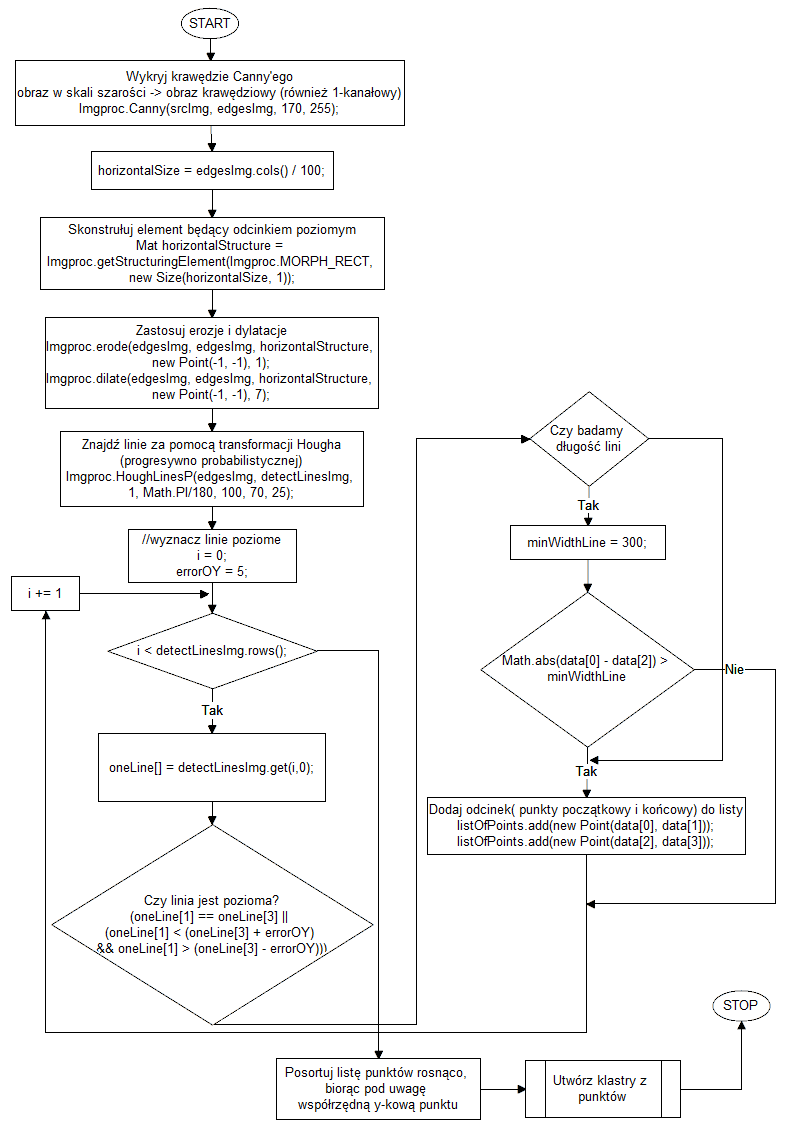
\includegraphics[height=23cm]{image//algorithm//prepareImgToAnalize.png} 
    			    \end{center}
    		    	\caption
        	    		[Algorytm znajdujący linie poziome]  
            			{Algorytm znajdujący linie poziome}  
    		    \end{figure}	
				
    			\begin{figure}[!ht]  
    		        \begin{center}
    		    	    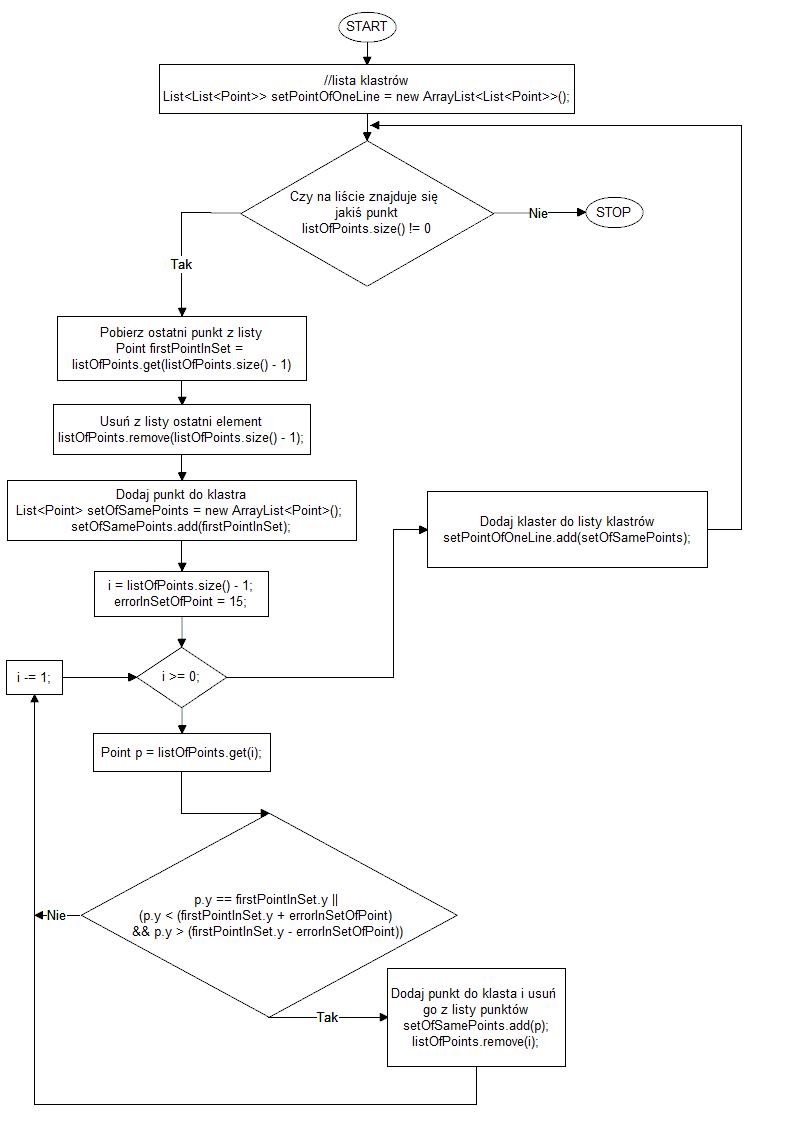
\includegraphics[height=22.5cm]{image//algorithm//prepareImgToAnalizePred.png} 
    			    \end{center}
        			\caption
        			    [Algorytm budujący listę klastrów]  
            			{Algorytm budujący listę klastrów}  
    		    \end{figure}
		        \newpage
		        Algorytm wykorzystuje zasadnicze przekształcenia morfologiczne udostępnione w bibliotece OpenCv --- dylatacje i erozje, które mają szerokie zastosowanie w zagadnieniu przetwarzania obrazów. \par
		        Dylatacja jest to konwolucja obrazu i jądra, w której wszystkie piksele zostają zastąpione na lokalne maksimumm każdego z pikseli, które obejmuje jądro. Jest to operacja nieliniowa, która powoduje rozrastanie się jasnego obszaru i zazwyczaj powoduje wypełnienie zagłębień przy przyjęciu założenia, że jądro jest jądrem wypukłym i wypełnionym. \par
    		    Erozja jest to operacja przeciwna do operacji dylatacji, a więc piksele zostają zastąpione na lokalne minimum, jest to również operacja nieliniowa, która powoduje zmniejszenie się czarnego obszaru oraz usuwa wypukłości, przy tych samych założeniach.
		    
		\subsubsection{Wyprostowanie strony}		
		    \paragraph{\indent} 
		    Metody klasy ToStraightenUp pomagają zniwelować w pewnym stopniu wpływ      ludzki na jakość przetwarzania obrazu. Umożliwiają one wyprostowanie        danego zdjęcia jeśli zostało ono niewłaściwie, krzywo umieszczone na      skanerze. Klasa ta wykorzystuje również metody klasy PrepareImgToAnalize     dzięki której buduje zbiór linii, z których każda ma taką podobną           współrzędną y---kową początku i końca. I na podstawię średniej z różnic     tej współrzędnej wykrytych linii określany jest kąt o jaki należy        obrócić obraz, tak aby został on wyprostowany.  
		
		        Algorytm wykorzystuje funkcję zaimplementowaną w bibliotece OpenCv przekształcającą obraz. Jest to funkcja przekształcenia afinicznego:
    		    \begin{center}
    		        \textit{Imgproc.warpAffine(srcImg, dstImg, M, dsize);}.
    		    \end{center}
		    
		        która punkt macierzy źródlowej \textit{srcImg} przekształca do macierzy wynikowej \textit{dstImg} według macierzy określającej jakiego rodzaju jest to przeształcenie \textit{M} mającej dwa wiersze i trzy kolumny według nastepującego wzoru:
                \begin{center}
                    \textit{$dst(x,y) = src( M_{11} x + M_{12} y + M_{13}, M_{21} x + M_{22} y + M_{23}$}.
                \end{center} \par    
                Ponieważ prawa strona równania często nie jest liczbą całkowitą, wartość odpowiedniego punktu macierzy wynikowej oblicza się stosując interpolację. Metoda ta dostarcza również innych wariantów wywołania z kolejnymi argumentami takimi jak: 
                \newpage
                \begin{spacing}{\spacingInSimpleItemize}
                \begin{itemize}
                    \item \textit{flags} --- wybór metody interpolacji, 
                    dostępne są następujące typy:\\
                   
                    \begin{itemize}
                    \item INTER\_NEAREST --- najbliższego sąsiada,\\ 
                    \item INTER\_LINEAR --- dwuliniowa,\\
                    \item INTER\_AREA --- przepróbkowanie obszaru pikseli,\\
                    \item INTER\_CUBIC --- interpolacja dwusześcianowa,\\
                    \begin{spacing}{\spacingInSolemnItemize}
                    \item INTER\_LANCZOS4 --- interpolacja wykorzystująca metodę Lanczosa biorąca pod uwagę sąsiednie punkty w obszarze o wymiarach 8x8,\\ 
                    można dołączyć dodatkową opcję przy użyciu operatora lub WRAP\_INVERSE\_MAP --- przekształcenie z \textit{dstImg} do \textit{srcImg},
                    \end{spacing}
                    \end{itemize}
                     \begin{spacing}{\spacingInSolemnItemize}
                    \item \textit{borderMode} --- metoda użyta do ekstrapolacji pikseli znajdujących się na zewnątrz obrazu, dostępne są następujące typy:
                    \end{spacing}
                    
                    \begin{itemize}
                    \item BORDER\_CONSTANT --- dodaje piksele o stałej wartości,\\
                    \item BORDER\_WRAP --- dodaje piksele przez pobranie ich z przeciwnej strony,\\
                    \item BORDER\_REPLICATE --- dodaje piksele przez skopiowanie ich z krawędzi,\\
                    \item BORDER\_REFLECT --- dodaje piksele przez lustrzane odbicie,\\\begin{spacing}{\spacingInSolemnItemize}
                    \item BORDER\_REFLECT\_101 --- dodaje piksele przez lustrzane odbicie przy tym nie duplikując pikseli tworzących krawędź,\end{spacing}
                    \item BORDER\_DEFAULT --- jest to alias dla  BORDER\_REFLECT\_101,
                    \end{itemize}\begin{spacing}{\spacingInSolemnItemize}
                    \item \textit{borderValue} --- paramentr wżywany w przypadku stałej granicy, wartością domyślną jest zero.  
        		    \end{spacing}
        		 \end{itemize}
        		 \end{spacing}
		        \newpage
        		 \begin{figure}[!ht]  
                    \begin{center}
        	    	    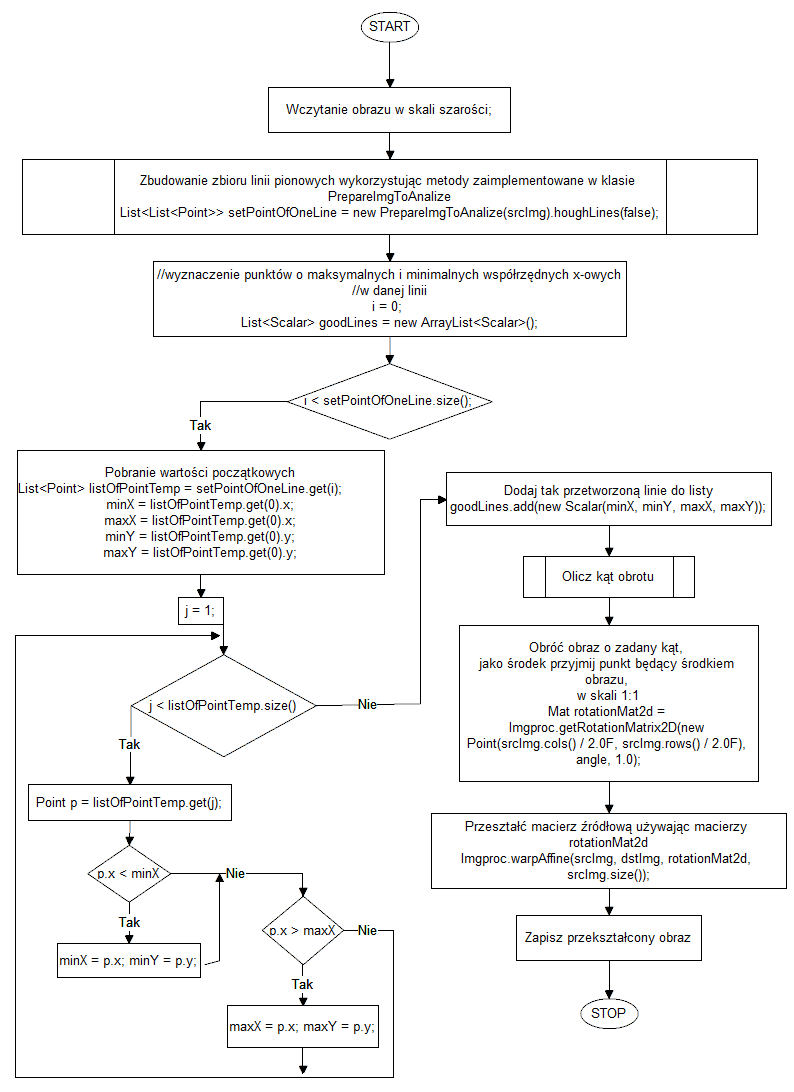
\includegraphics[height=22.5cm]{image//algorithm//toStraightenUp.png} 
    			    \end{center}
        		    \caption
            			[Algorytm obracający obraz tak aby był prosty]  
            			{Algorytm obracający obraz tak aby był prosty}  
        	    \end{figure}
        		 \newpage
    		    %\begin{figure}[!ht]  
                %   \begin{center}
        	         %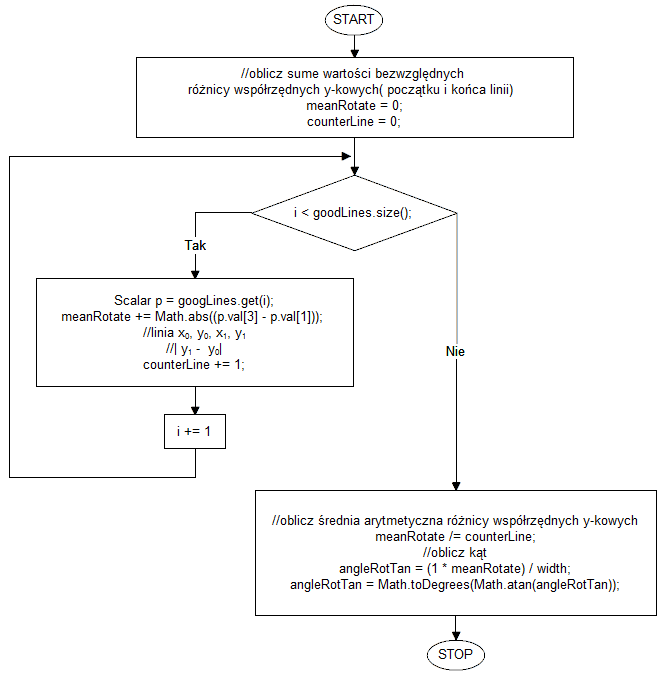
\includegraphics[height=12cm]{image//algorithm//toStraightenUpPred.png} 
    			    %\end{center}
        		    %\caption
        			 %   [Algorytm obliczający kąt obrotu]  
        			 %   {Algorytm obliczający kąt obrotu}  
        	    %\end{figure}
		    
		    \lstinputlisting[caption=Algorytm obliczający kąt obrotu]{calculateAngle.java}
        	
        		\begin{figure}[!ht]  
        		    \begin{center}
        			    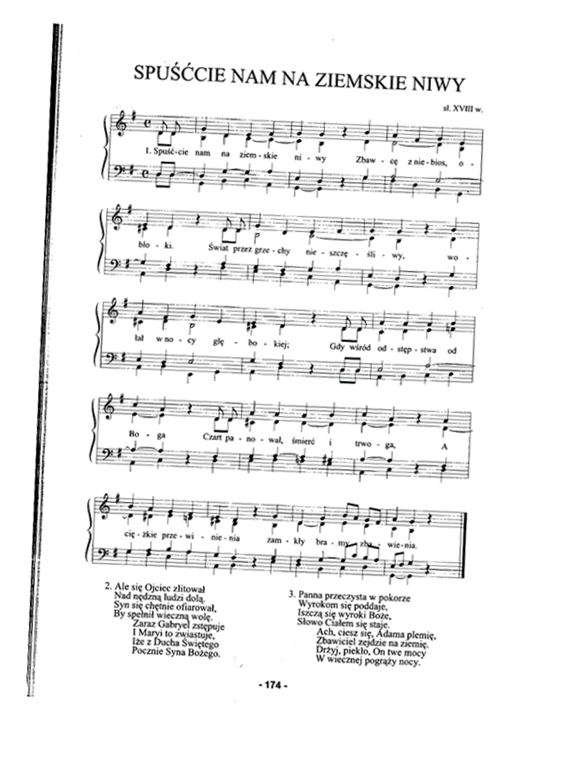
\includegraphics[height=17cm, frame]{image//exampleImage//003_a.png} 
        		    \end{center}
        		    \caption
        			    [Obraz przed wyprostowaniem]  
            			{Obraz przed wyprostowaniem}  
        	    \end{figure}
        			
                \begin{figure}[!ht]  
        		    \begin{center}
        			    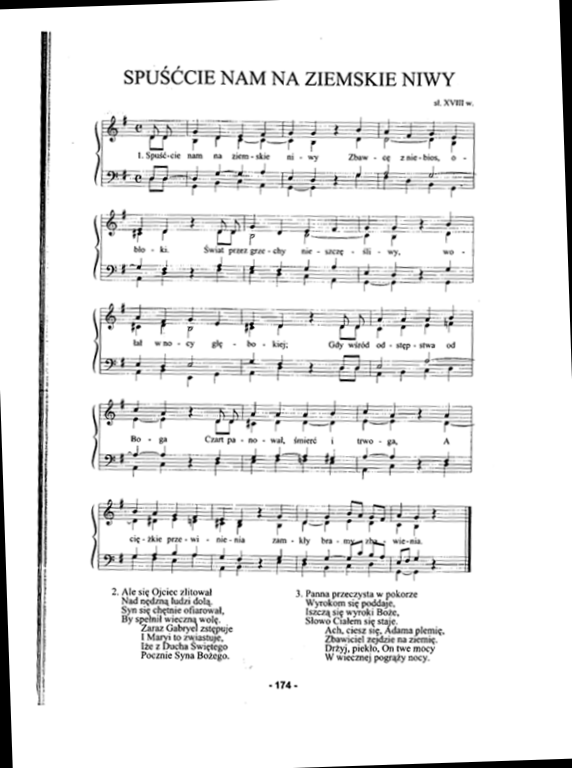
\includegraphics[height=17cm, frame] {image//exampleImage//003_b.png} 
        		    \end{center}
        			\caption
            			[Obraz po wyprostowaniu]  
            			{Obraz po wyprostowaniu}  
        	    \end{figure} 
		
		        \newpage 
		 
	    \subsubsection{Główne przetwarzanie obrazu}
		    \paragraph{} Metody klasy MajorProcessing również używają algorytmów zaimplementowanych     w klasie PrepareimgToAnalize. Wykryte linie transformatą Hougha zostają     pogrupowane w zbiory tworzące pięciolinie. Odpowiednio w zależności od      budowy śpiewnika z jedna pięciolinią (klucz wiolinowy) z tekstem            umieszczonym pod nią lub z dwiema pięcioliniami oraz tekstem umieszczonym     pomiędzy nimi. Następnie wykryte pięciolinie zostają zamarkowane             utwarzając bounding boxy i wraz z tekstem znajdującym się pod lub między     nimi wycięte z obrazu i zapisane do osobnych plików czy macierzy            przechowujących obrazy, a więc przygotowane do dalszego przetworzenia i     ostatecznego uzyskania z nich tekstu.
		
			\begin{figure}[!ht]  
			    \begin{center}
				    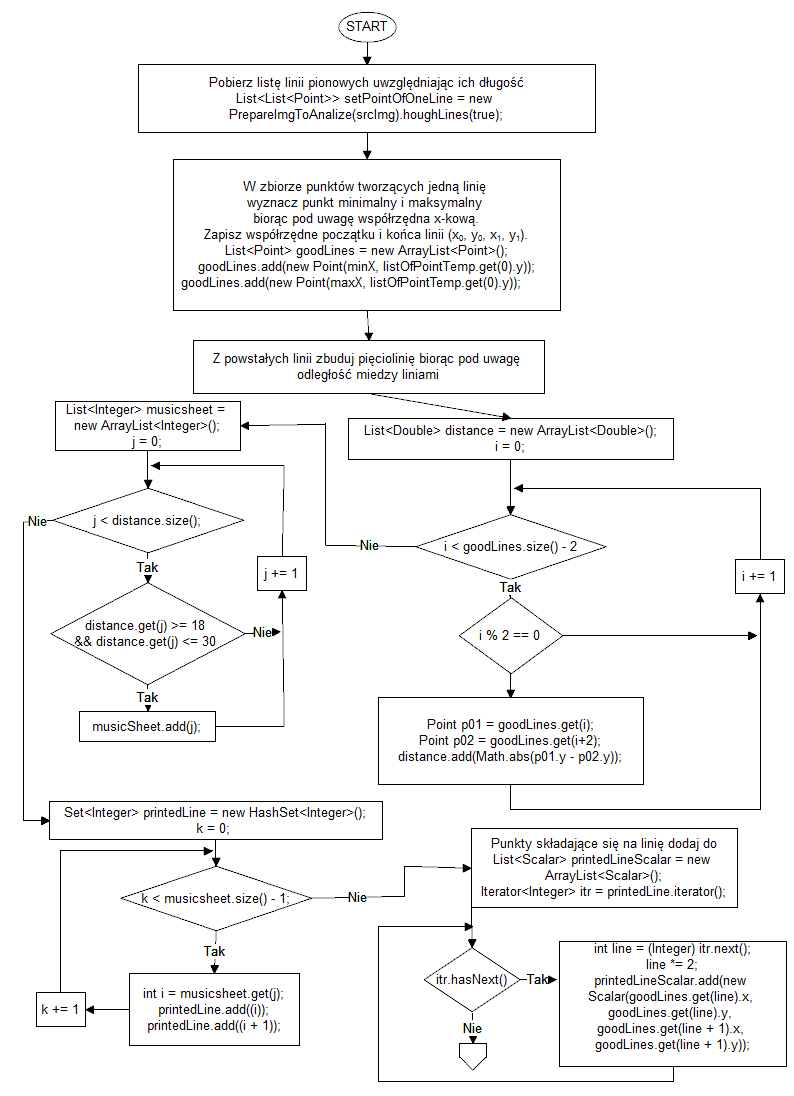
\includegraphics[height=22.5cm]{image//algorithm//majorProcesing_01.png} 
			    \end{center}
			    \caption
    			    [Główny algorytm budujący bounding boxy cz. 1]  
    			    {Główny algorytm budujący bounding boxy cz. 1}  
		    \end{figure}
			
			\newpage
			
	        \begin{figure}[!ht]  
			    \begin{center}
				    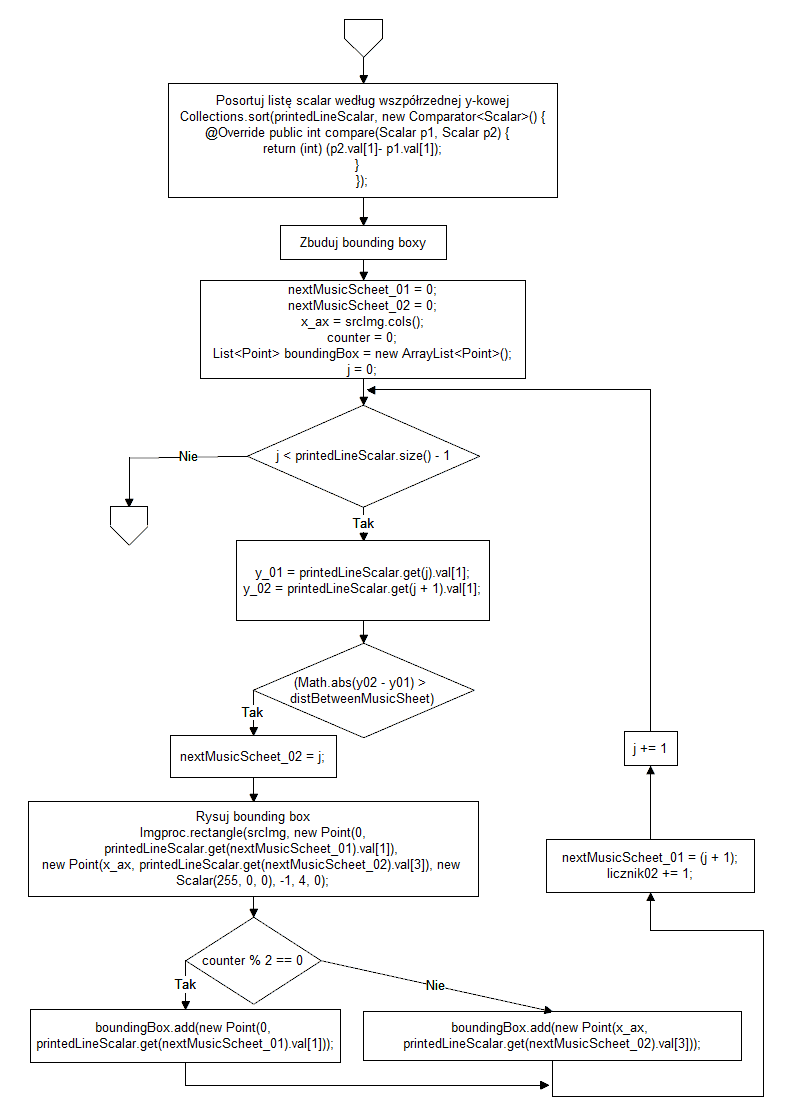
\includegraphics[height=23cm] {image//algorithm//majorProcesing_02.png} 
			    \end{center}
			    \caption
    			    [Główny algorytm budujący bounding boxy cz. 2]  
    			    {Główny algorytm budujący bounding boxy cz. 2}  
		    \end{figure} 
		
		    \begin{figure}[!ht]  
			    \begin{center}
				    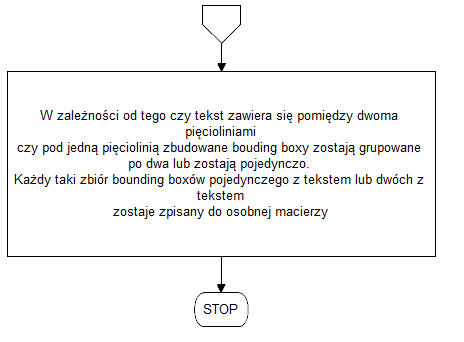
\includegraphics[height=8cm] {image//algorithm//majorProcesing_03.png} 
			    \end{center}
			    \caption
    			    [Główny algorytm budujący bounding boxy cz. 3]
    			    {Główny algorytm budujący bounding boxy cz. 3}  
		    \end{figure} 
		
    		\begin{figure}[!ht]  
			    \begin{center}
				    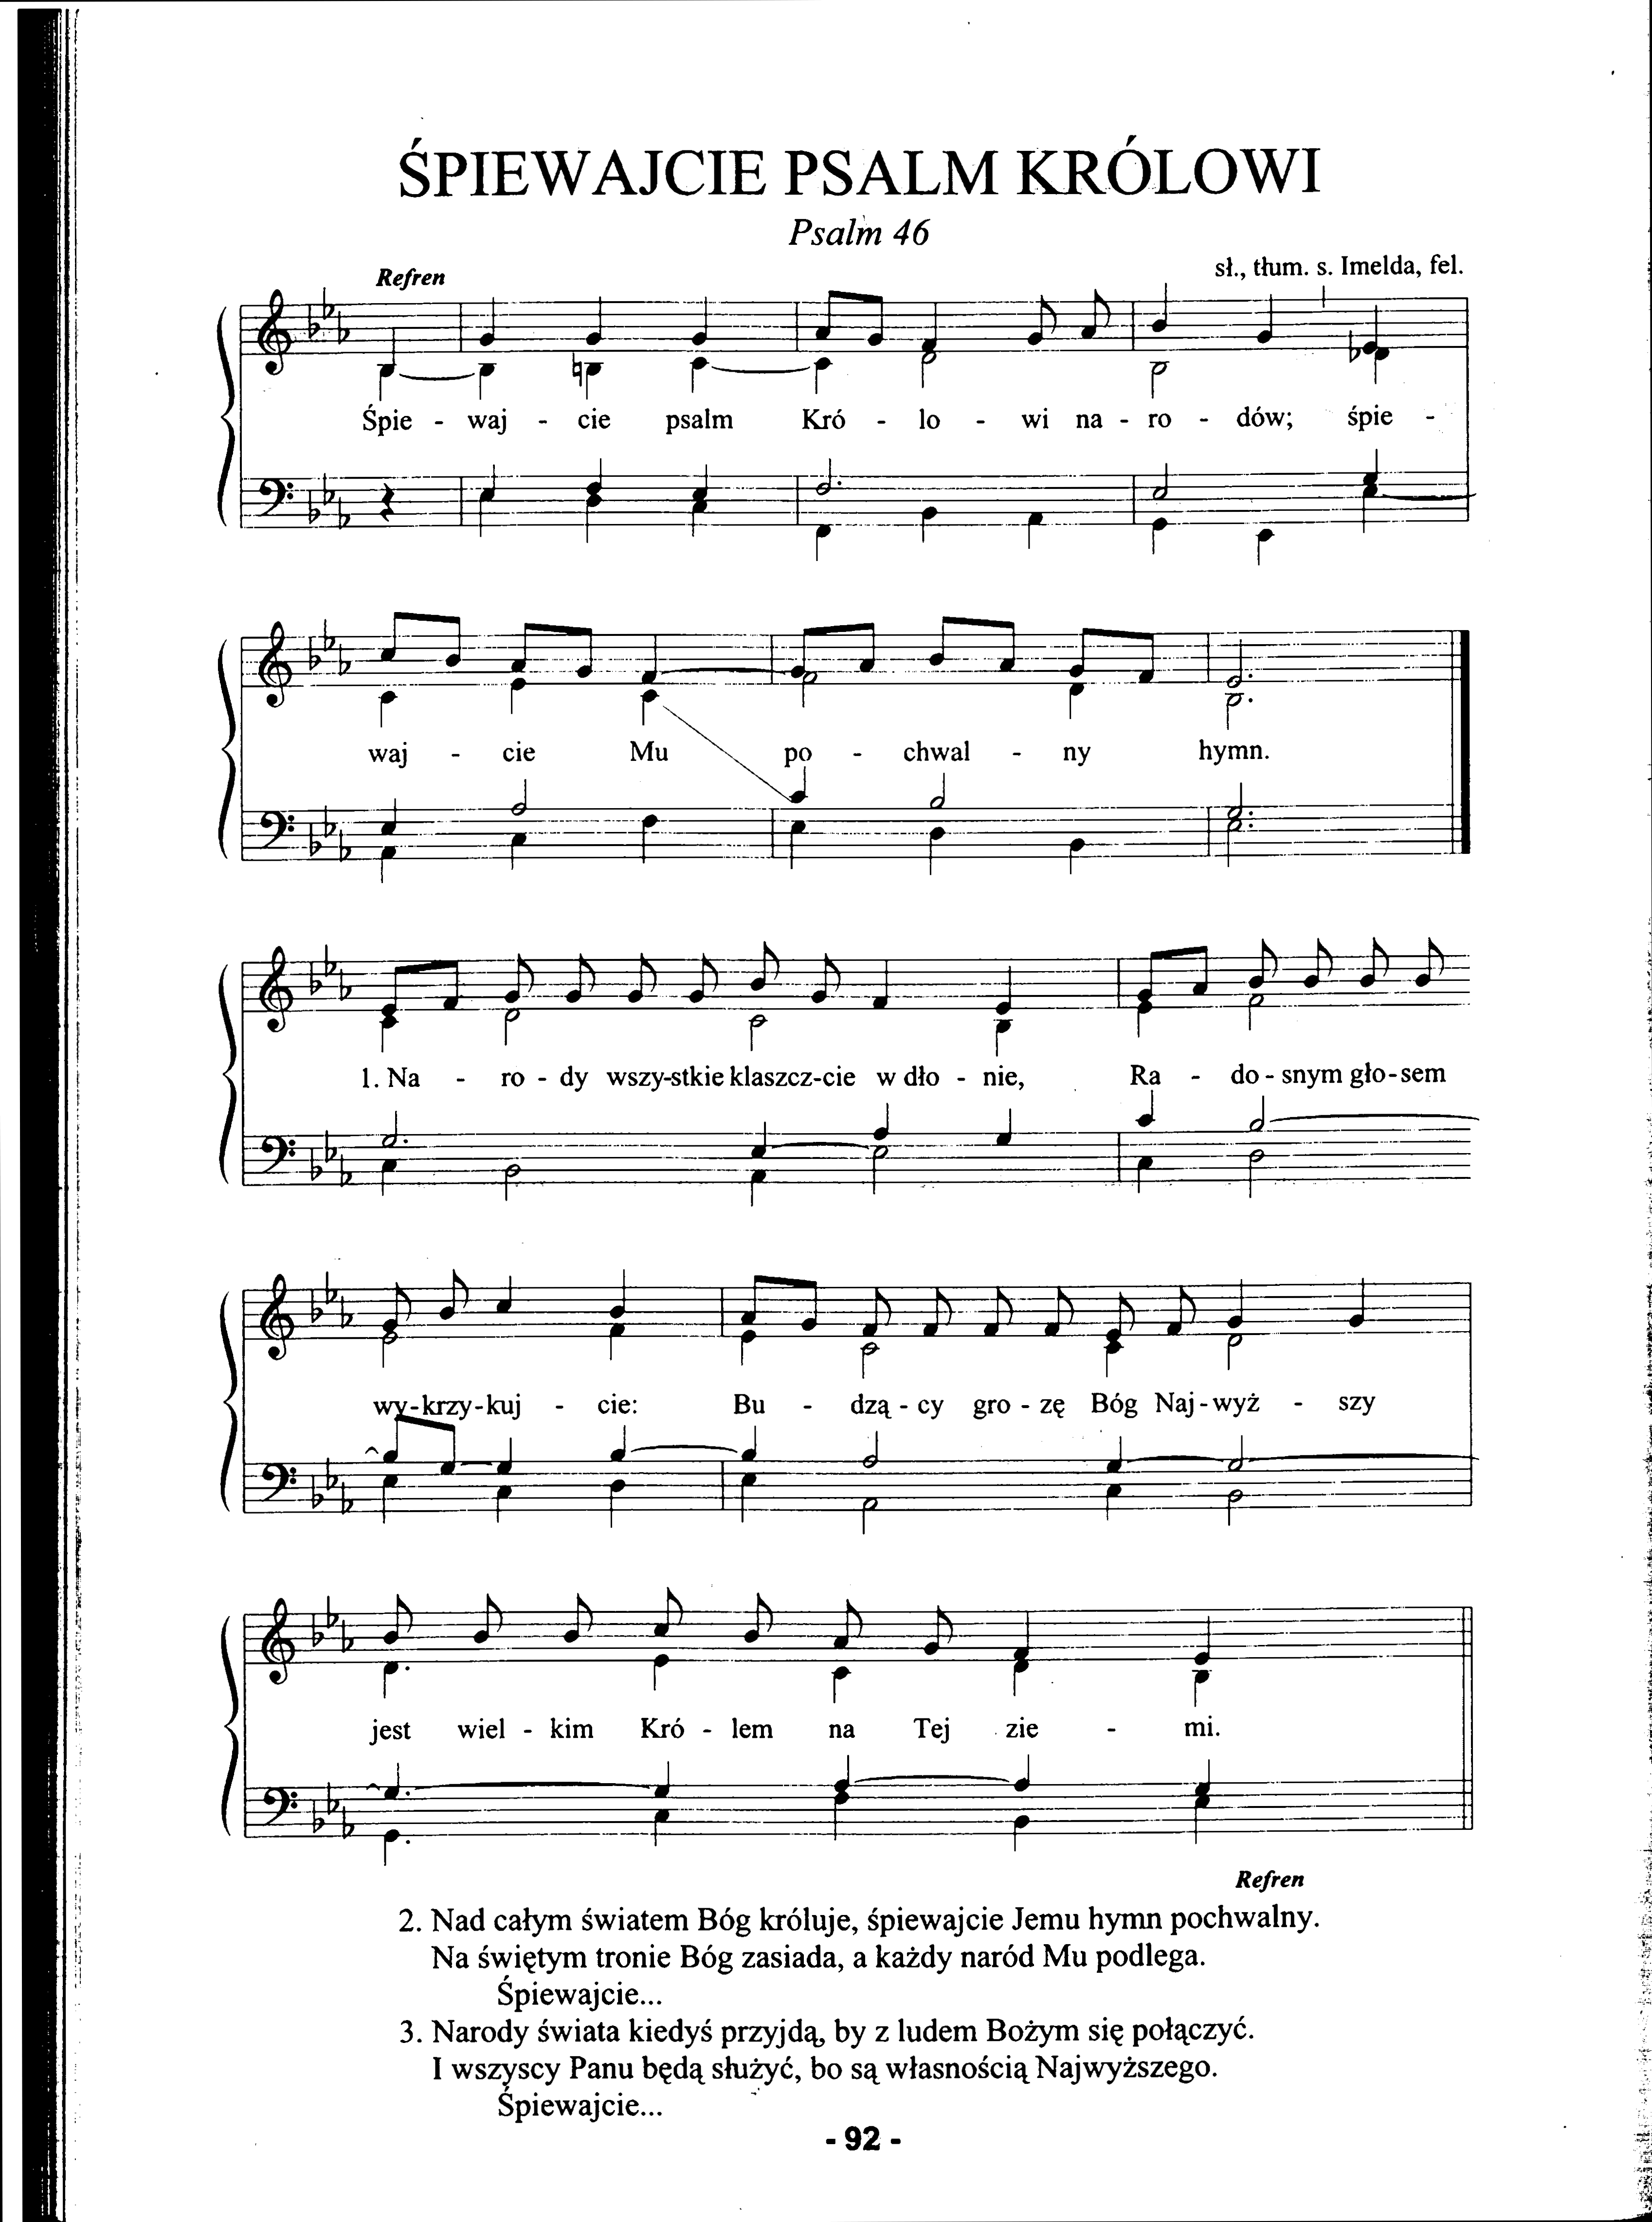
\includegraphics[height=13cm, frame] {image//exampleImage//004_a.png} 
			    \end{center}
			    \caption
    			    [Obraz przed wykryciem pięciolinii]  
    			    {Obraz przed wykryciem pięciolinii}  
		    \end{figure} 
		
		    \begin{figure}[!ht]  
			    \begin{center}
				    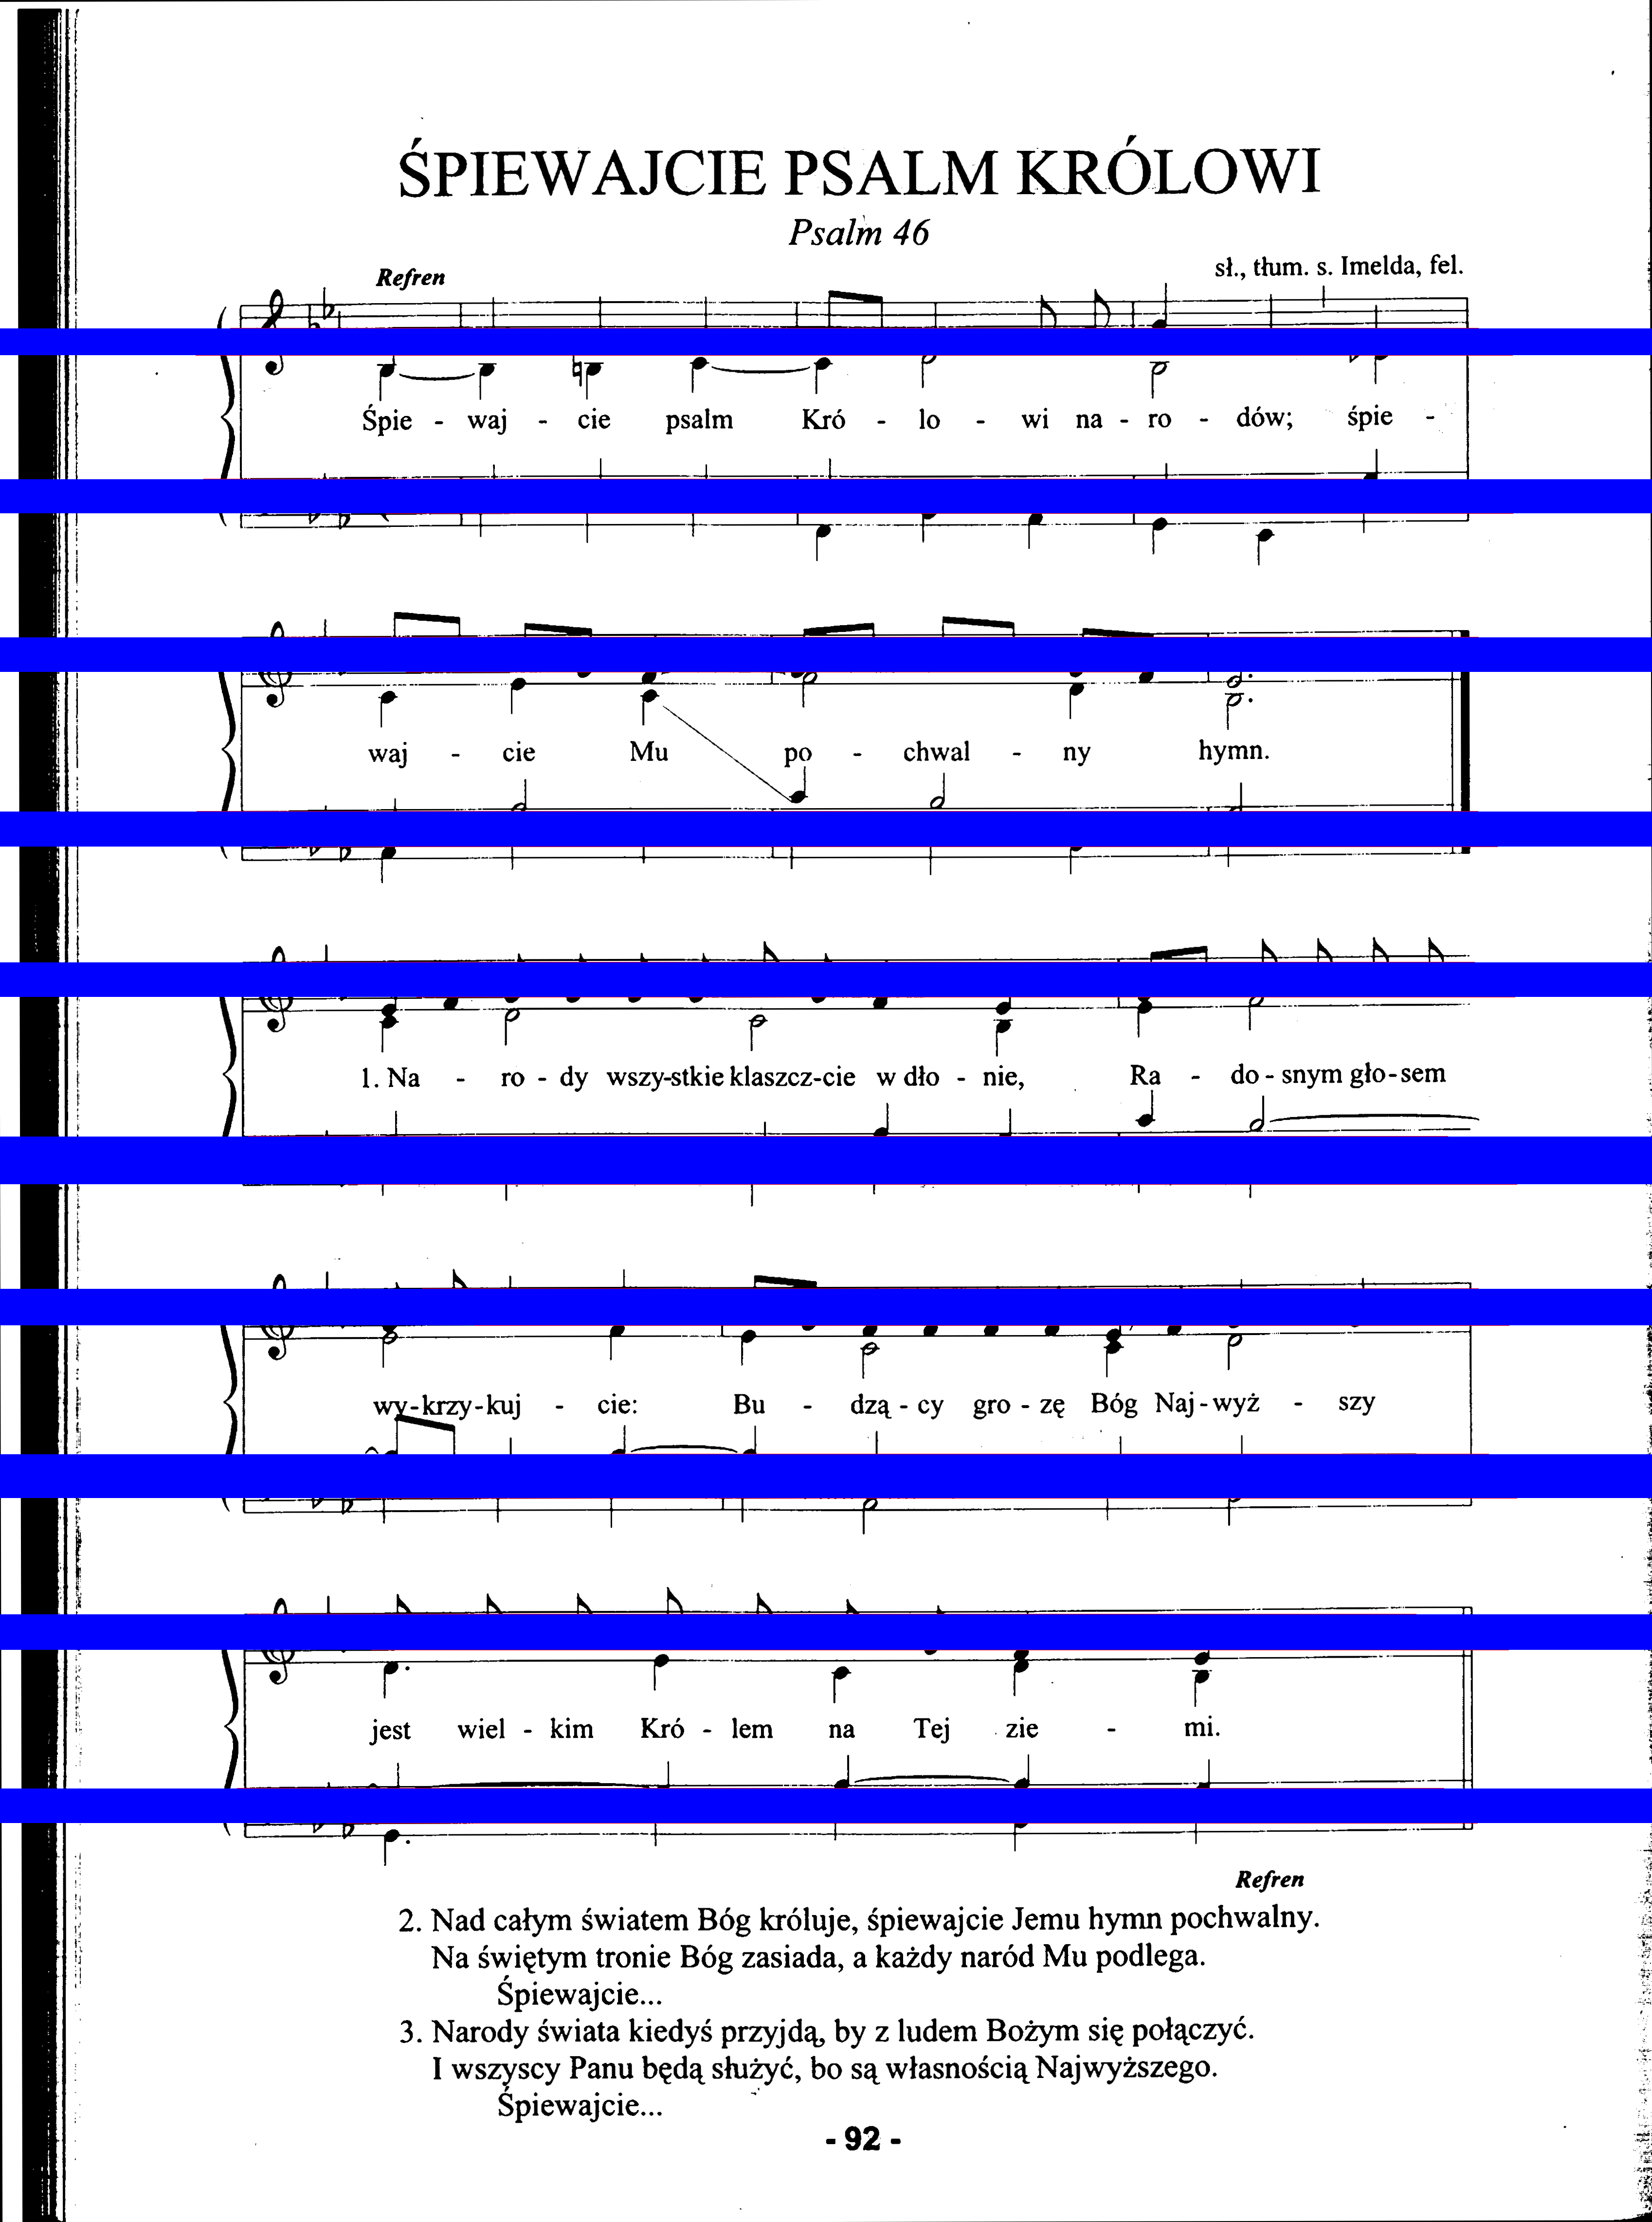
\includegraphics[height=15cm, frame] {image//exampleImage//004_b.png} 
			    \end{center}
			    \caption
    			    [Obraz po wykryciu pięciolinii]  
    			    {Obraz po wykryciu pięciolinii}  
		    \end{figure} 
		
		\subsubsection{Konfiguracja sieci neuronowej klasyfikującej linię}  
	        \paragraph{\indent} Klasa MusicSheetClassifier zawiera model konwolucyjnej sieci neuronowej który           zostaje nauczony klasyfikacji obrazów wejściowych na zawierające        tekst lub  pięciolinię, na podstawie wcześniej przygotowanych zdjęć         treningowych (jednokanałowych, o roazmiarzach 600px x 15px).
	        \newpage
		
    		%\begin{figure}[!ht]  
	    	%    \begin{center}
	        %		    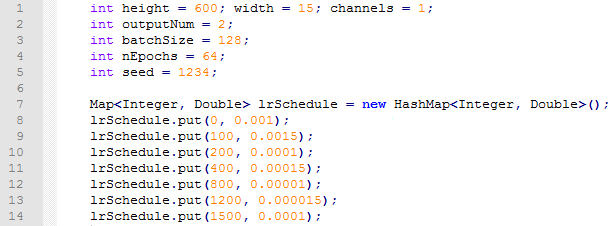
\includegraphics[width=15cm, frame] {image//practicalPart//cnnConf_03.png} 
	    	%    \end{center}
		    %\end{figure}
                
	        %\begin{figure}[!ht]  
    		%    \begin{center}
    		%	    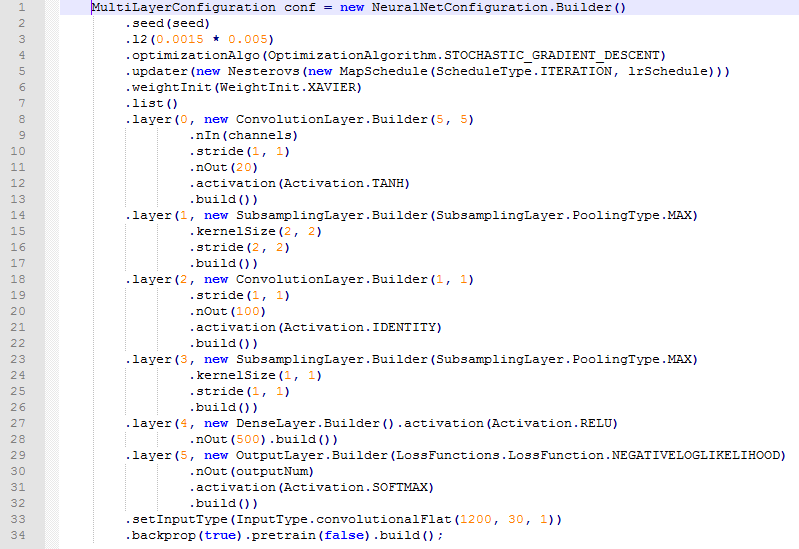
\includegraphics[width=15cm, frame] {image//practicalPart//cnnConf_04.png} 
    		%    \end{center}
		    %\end{figure}  
		
		    \lstinputlisting[caption=Konfiguracja sieci neuronowej klasyfikującej linię]{cnnMusicSheet.java}
		
            \begin{spacing}{\spacingInSolemnItemize}
		    \begin{center}
                \begin{tabular}{c c c }
                    \# of classes: & liczba klas & 2 \\
                    Accuracy:  & dokładność &0,9806  \\ 
                    Precision:  & precyzja & 0,9768 \\  
                    Recall: & wycofanie & 0,9808      \\
                    F1 Score: & rezultat f1 & 0,9851
                \end{tabular}
            \end{center}
		    \end{spacing}

%                \item optimizationAlgo - algorytm optymalizacji dotyczy działania p%arametrów określonych w updater. Stochastic gradient descent wykonuje optymalizację, której celem jest znalezienie maksimum w danym przedziale. Optymalizacja obejmuje obliczenie wartości błędu i zmianie wag w celu osiągnięcia minimalnego błędu;
  %              \item updater - określa współczynniki uczenia się sieci;
   %             \item weightInit - inicjalizacja wag sieci neuronowej. Xavier jest zazwyczaj właściwym parametrem, aby zainicjowane wagi nie były zbyt duże ani zbyt niskie;
            
%                \item DenseLayer.Builder() - warstwa przetwarzająca wszzystkie wyniki z warstwy poprzedniej; 
                %\item OutputLayer.Builder(LossFunctions.LossFunction.NEGATIVELOGLIKELIHOOD) - wyjściowa warstwa ukryta z okreslona funkcja straty.
		
		\subsubsection{Detekcja tekstu} 		
			\paragraph{\indent} Algorytmy zaimplementowane w klasie DetectText umożliwiają w              dotychczas przygotowanych obrazach, maksymalnie rozszerzyć obszar           powstałych bounding boxów na podstawie odchylenia standardowego, co       umożliwia praktycznie całkowite usunięcie znaków muzycznych (nut i        pięciolinii). Obszar w którym prawdopodobnie znajduje się tekst zostaje     wycięty i jest obrazem wejściowym dla konwolucyjnej sieci neuronowej        która podejmuje decyzje czy jest on linią tekstu czy nut. Jeśli sieć        zwróci wartość pozytywną (obraz jest tekstem; prawdopodobieństwo wieksze     niż 0.9), zostaje on wycięty i poddany dalszej obróce, zaś jeśli sieć       zwróci wartość negatywną (obraz nie jest tekstem; prawdopodobieństwo        mniejsze lub równe 0.9) dalszemu przetwarzaniu zostaje poddany cały         obraz.  

			    \begin{figure}[!ht]  
			        \begin{center}
				        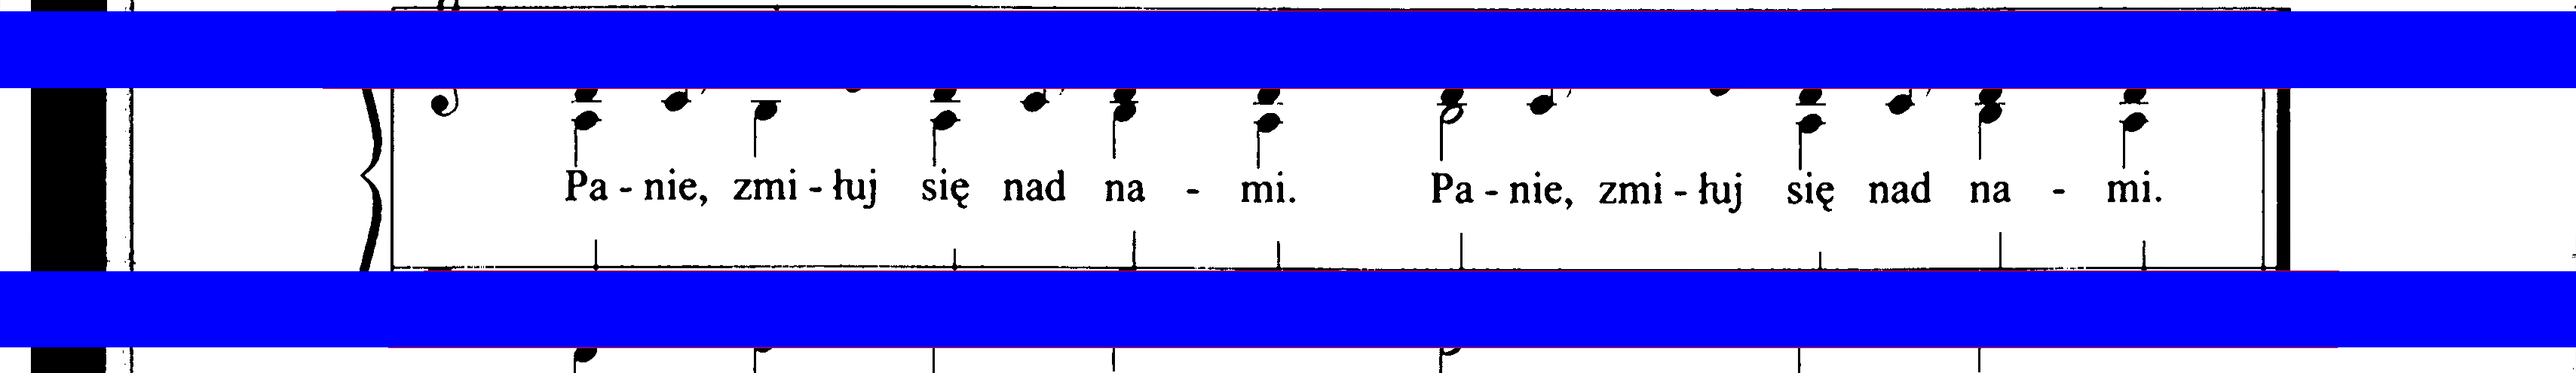
\includegraphics[width=16.5cm, frame] {image//exampleImage//005_a.png} 
			        \end{center}
			        \caption
    			        [Obraz przed rozszerzeniem bounding boxów]  
    			        {Obraz przed rozszerzeniem bounding boxów}  
		        \end{figure} 
		
		        \begin{figure}[!ht]  
			        \begin{center}
				        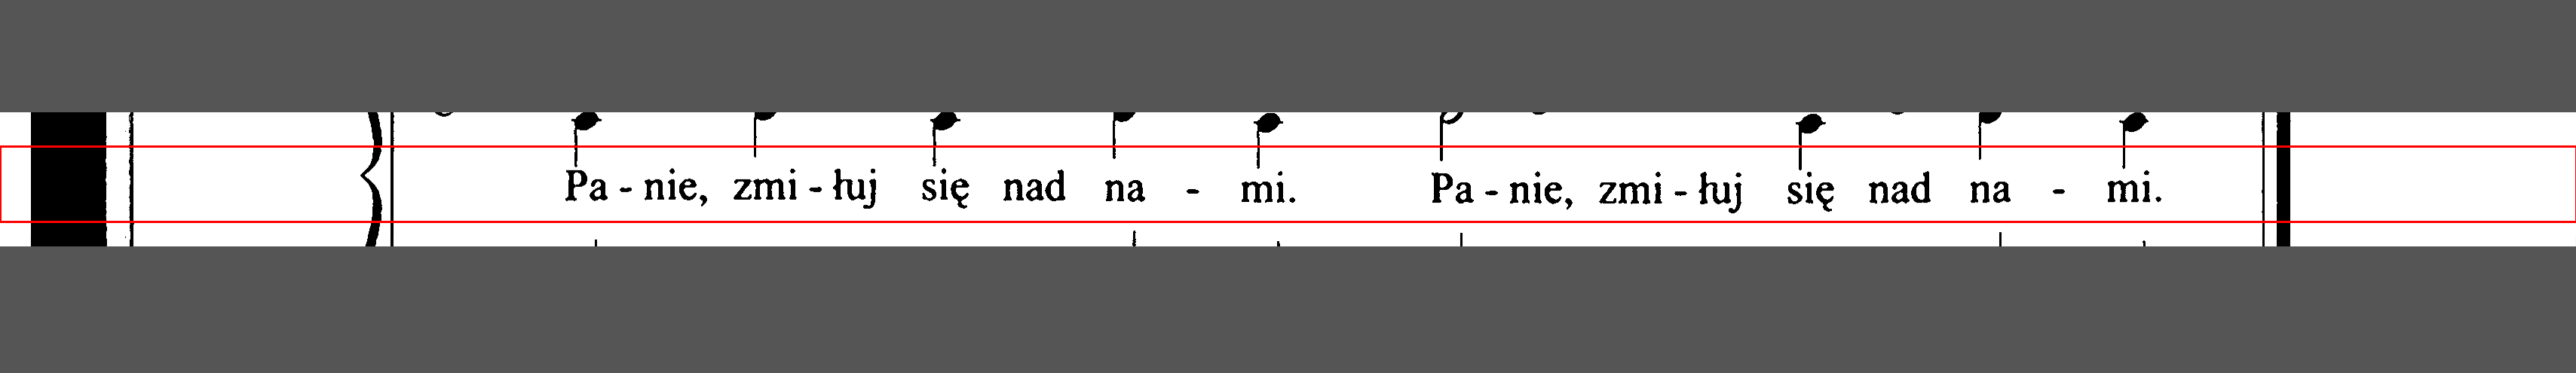
\includegraphics[width=16.5cm, frame] {image//exampleImage//005_b.png} 
			        \end{center}
			        \caption
    			        [Obraz po rozszerzeniu bounding boxów i zamarkowaniu miejsca gdzie znajduje się tekst]  
    			        {Obraz po rozszerzeniu bounding boxów i zamarkowaniu miejsca gdzie znajduje się tekst}  
		        \end{figure} 
		    \newpage
		        \begin{figure}[!ht]  
			        \begin{center}
				        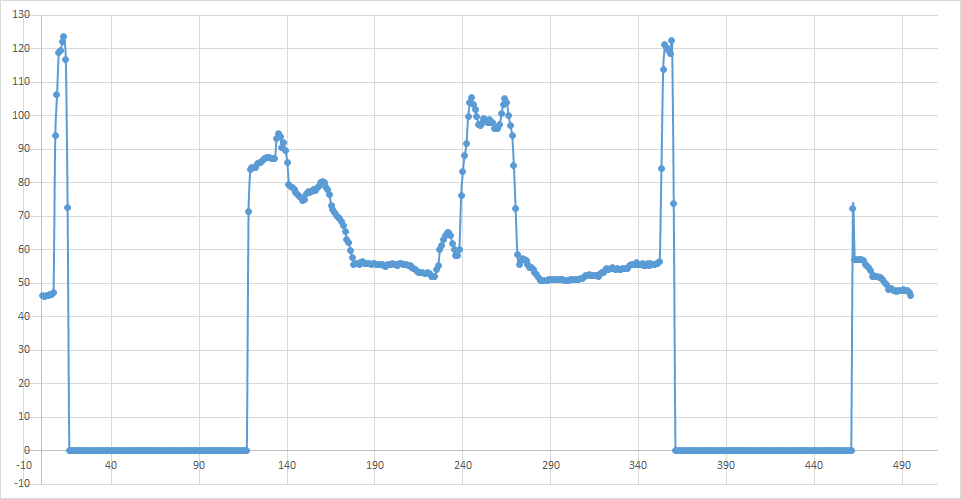
\includegraphics[height=9cm, frame] {image//practicalPart//stdDevDetectText.png} 
			        \end{center}
			        \caption
        			    [Wykres odchylenia standardowego poszczególnych linii]  
        			    {Wykres odchylenia standardowego poszczególnych linii}  
		        \end{figure}
		    
		    Na podstawie wykresu można zauważyć ze tekst znajduje się pomiędzy dwoma większymi obszarami o wartościach zerowych, dokładniej pomiędzy liniami od około 240 do około 270, odchylenie standardowe wierszy zawierających tekst waha się w zakresie od około 95 do około 105. Obszar pomiędzy tekstem a zamarkowanymi pięcioliniami ma niezbyt duże odchylenie standardowe ponieważ mogą się w tych liniach znajdować nuty dodane, ogonki nut jednak nie będzie ich nigdy zbyt wiele i rozrzut w tych liniach nie będzie większy od rozrzutu w liniach w których znajdują się litery.

        \subsubsection{Detekcja i wycięcie liter}
            \paragraph{\indent} Algorytmy kalsy DetectLetter wykrywają krawędzie w obrazie wejściowym,     następnie grupują je w zbiory o taki samych współrzędnych x-owych, dzięki    czemu jedna grupa konturów stanowi jeden znak (literę, znak                 interpunkcyjny, etc.), grupy są sortowane rosnąco według współrzednych      x-owych. Z każdego zbioru konturów zostają wyznaczone skrajne współrzędne    $ max_{x} , min_{x}, max_{y}, min_{y} $. Na podstawie tych wartości z       obrazu wejsciowego zostaje wycięty kontur zawierający się w tym             prostokącie. Tak wyciętemu obrazowi zostaje nadana jednoznaczna nazwa       według jego indeksu w zbiorze posortowanym, według rosnącego rozmieszczenia w osi x obrazu. 
    
            \begin{figure}[h!]
                \centering
                \begin{subfigure}[b]{2cm}
                    
\includegraphics[width=1.5cm, height=1.5cm, frame]{image//exampleImage//letter_01.png}
                    \caption{}
                \end{subfigure}
                \begin{subfigure}[b]{2cm}
                    
\includegraphics[width=1.5cm, height=1.5cm, frame]{image//exampleImage//letter_02.png}
                \caption{}
                \end{subfigure}
                \newline
                \begin{subfigure}[b]{2cm}
                    
\includegraphics[width=1cm, height=2cm, frame]{image//exampleImage//letter_03.png}
                    \caption{}
                \end{subfigure}
                \begin{subfigure}[b]{2cm}
                    
\includegraphics[width=1cm, height=2cm, frame]{image//exampleImage//letter_04.png}
                    \caption{}
                \end{subfigure}
                \caption
                [Przykladowe wycięte litery]
                {Przykladowe wycięte litery}
                %\label{}
            \end{figure}

        \subsubsection{Konfiguracja sieci neuronowej klasyfikującej litery}
            \paragraph{\indent} Klasa LetterClassifier zawiera model konwolucyjnej sieci neuronowej który           zostaje nauczony rozpoznawania liter abecadła, w tym polskich znaków     diakrytycznych, majuskuł i minuskuł (łącznie 64 znaki, klasy), na           podstawie wcześniej przygotowanych zdjęć treningowych (jednokanałowych,     o rozmiarach 50px x 25px), Konfiguracja sieci różni się od poprzedniej     jedynie kilkoma parametrami i dodatkowymi dwoma warstwami:                  ConvolutionLayer.Builder(x, y) i 
                SubsamplingLayer.Builder(SubsamplingLayer.PoolingType.MAX).
	       
	       
	       \lstinputlisting[caption=Konfiguracja sieci neuronowej kalsyfikującej litery]{cnnLetter.java}
	       
	       
	            %\begin{figure}[!ht]  
	    	    %    \begin{center}
	    		%        \includegraphics[width=15cm, frame] %image//practicalPart//cnnConf_01.png} 
	    	    %    \end{center}
		        %\end{figure}
            
	            %\begin{figure}[!ht]  
    		    %    \begin{center}
    			%        \includegraphics[width=15cm, frame] %{image//practicalPart//cnnConf_02.png} 
    		    %    \end{center}
		        %\end{figure}            

            Trening sieci neuronowej daje dość zadowalające wyniki 
    
            \begin{spacing}{\spacingInSolemnItemize}
                \begin{center}
                \begin{tabular}{ c c c  }
                    \# of classes: &  liczb klas & 64 \\
                    Accuracy:  & dokładność & 0,7387  \\ 
                    Precision:  & precyzja & 0,7098 \\  
                    Recall: & wycofanie & 0,5776      \\
                    F1 Score: & rezultat f1 & 0,6347
                \end{tabular}
                \end{center}
            \end{spacing}
            
            Sieć bardzo dobrze rozpoznaje (zwraca wysokie prawdopodobieństwo > 0.9) pojedyncze litery podobne do tych ze zbioru na których się uczy. Podczas pracy ze zbiorem danych ze śpiewników nie zawsze algorytm rozpoznawania konturów pojedynczych liter zwraca zadowalające wyniki (same pojedyncze litery) często gdy kontury liter zachodzą na siebie zwraca kilka liter w jednym obrazie lub dodatkowych znaków co uniemożliwia poprawne rozpoznanie przez sieć. 

            \begin{figure}[h!]
                \centering
                \begin{subfigure}[b]{2cm}
                    
\includegraphics[frame]{image//practicalPart//w_letter_01.png}
                \caption{}
                \end{subfigure}
                \begin{subfigure}[b]{2cm}
                    
\includegraphics[frame]{image//practicalPart//w_letter_02.png}
                \caption{}
                \end{subfigure}
              \newline
                \begin{subfigure}[b]{2cm}
                    
\includegraphics[frame]{image//practicalPart//w_letter_03.png}
                \caption{}
                \end{subfigure}
                \begin{subfigure}[b]{2cm}
                    
\includegraphics[frame]{image//practicalPart//w_letter_04.png}
                    \caption{}
                \end{subfigure}
                \caption
                    [Przykladowe znaki, litery wycięte niepoprawnie]
                    {Przykladowe znaki, litery wycięte niepoprawnie}
                %\label{}
            \end{figure}

        \subsubsection{Klasyfikacja odczytanych liter}
	        \paragraph{\indent} Algorytmy kalsy ReadLetterClassifier odczytują przygotowany     przez klasę DetectLetter obraz zawierający znak, następnie obraz ten        zostaję analizowany przez system OCR Tesseract oraz konwolucyjną sieć       neuronową. Wybranie najbardziej prawdopodobnej litery odbywa się przez      porównanie wyniku zwróconego przez system OCR i trzech największych         prawdopodobieństw zwróconych przez sieć. Tak odczytany cały wykryty         tekst znajdujący się na stronie zostaje zapisany do pliku tekstowego.
	        
	            Przykładowy odczytany tekst: \textbf{Nie wiem czy jednak umieszczać ten przykładowy tekst :)}
	        
	         "lLH HŁ»» gzFłI—I„=iChwałaTobiesłowoBożechwałaTobiesłowoBożeIłłełt»\\
	         ————~„AA    BtChnenwCue    wałaTobiesłowoBoże 222121ałaTobiesłowoBoże\\
	         ›ie   S5łlłowoBożechwałaTobie›”J«eui;IW7~LA   FLFA   CI\\   W„chwałaTobie„ł3i  hia      lłłaTobie„u    i„«——IIsłowoBo\\ EIOWOAj0Boze „uiB  n„   l›    H;1N ki\\ DJllAllelujaallelu—jazJJA;JJtl   AllJ      elui       „›\\ 
	         Iall lelujaA  thJ     j FJr      I—"  
	        
	        
	   \newpage  
	   \section{Podsumowanie}
	   \paragraph{\indent} W niniejszej pracy dyplomowej zostały zrealizowane główne jej założenia. Opracowane algorytmy umożliwiają pozyskanie tekstu ze stron zawierających znaki muzyczne. Wśród uzyskanego tekstu możemy odnaleźć poszczególne sylaby, a nie rzadko i wyrazy. Identyfikacją liter składających się na poszczególne wyrazy może zostać jeszcze polepszona, przede wszystkim przez wykorzystanie dokładniejszych algorytmów wycinających poszczególne litery, powiększenie zbioru liter (majuskuł, minuskuł) i linii (tekstu, pięciolinii) na których uczą się sieci neuronowe. Dzięki zastosowaniu sztucznej inteligencji opracowane algorytmy są bardziej uniwersalne i umożliwią pracę ze znacząca liczbą powszechnie wykorzystywanych śpiewników wpisujących się w następujące dwa schematy [pięciolinia tekst pięciolinia], [pięciolinia tekst]. Dzięki wytworzeniu oprogramowania zgodnie z zasadami programowania zorientowanego obiektowo, z łatwością możemy do powyższych dwóch struktur dodawać kolejne w różnych konfiguracjach na przykład [pięciolinia tekst pięciolinia pięciolinia]. 
	   \par Jednym z celów pracy, który nie został zrealizowany było budowa graficznego interfejsu użytkownika, jednak wybrana technologia i architektura systemu umożliwiają dość proste przejście z aplikacji konsolowej do aplikacji posiadającej przejrzysty i przyjazny dla użytkownika interfejs. 
	   \par Dzięki pracy nad budową aplikacji mogłem rozwinąć swoje zdolności algorytmiczne i programistyczne. Zapoznanie się z podstawami teoretycznymi systemów przetwarzających tekst, działania sztucznych sieci neuronowych, algorytmów przetwarzających obrazy oraz z narzędziami związanymi z tymi zagadnieniami --- Tesseract, OpenCv, DL4J pozwoliło autorowi na zdobycie i rozwój swojej wiedzy i umiejętności. \textbf{Umiejętności zdobyte podczas pisania pracy dyplomowej będą stanowiły ciekawą pozycję dla przyszłych pracodawców. \textit{nie wiem jak to lepiej ując ze to calkiem ciekawie moze sie prezentowac w cv}}
	   
	   \newpage
	   \section{Bibliografia}
	   \subsubsection*{Źródła książkowe:}
	   \begin{spacing}{1.5}
	   \begin{itemize}
	        \item Rączkowski F., Śpiewajmy Bogu, Płock, Hejnał, 2012;
	        \item Siedlecki J., Śpiewnik kościelny, Wyd. XL (poprawione), Kraków,
	        Instytut Teologiczny Księży Misjonarzy, 2011;
	        \item Kaehler A., Bradski G., OpenCV 3. Komputerowe rozpoznawanie obrazu w C++ przy użyciu biblioteki OpenCV, Gliwice, Helion, 2017;
	        \item Shanmugamani R., Deep Learning for Computer Vision, Birmingham, Packt Publishing, 2018
	   \end{itemize}
	   \end{spacing}
	   
	   \subsubsection*{Źródła internetowe:}
	   Data dostępu 2018.07.15
	   \begin{spacing}{1}
	   \begin{itemize}
            \item \href{https://opencv.org}{\url{https://opencv.org}}
            \item \href{https://docs.opencv.org//3.1.0//index.html}{\url{https://docs.opencv.org//3.1.0//index.html}}
            \item \href{https://docs.opencv.org//java//3.1.0}{\url{https://docs.opencv.org//java//3.1.0}}
            
            \item \href{http://tess4j.sourceforge.net}{\url{http://tess4j.sourceforge.net}}
            
            \item \href{https://deeplearning4j.org//index.html}{\url{https://deeplearning4j.org//index.htmlt}}
            \item \href{https://nd4j.org//doc}{\url{https://nd4j.org//doc}}
            \item \href{https://depiesml.wordpress.com//category//deeplearning4j}{\url{https://depiesml.wordpress.com//category//deeplearning4j}}

            \item \href{https://ksopyla.com//python//operacja-splotu-przetwarzanie-obrazow}{\url{https://ksopyla.com//python//operacja-splotu-przetwarzanie-obrazow}}
            \item \href{https://github.com//Kulbear//deep-learning-nano-foundation//wiki//ReLU-and-Softmax-Activation-Functions}{\url{https://github.com//Kulbear//deep-learning-nano-foundation//wiki}}
            %https://github.com/Kulbear/deep-learning-nano-foundation/wiki/ReLU-and-Softmax-Activation-Functions

            \item \href{http://www.szkolazpasja.pl//rastrowa}{\url{http://www.szkolazpasja.pl//rastrowa}}
	   \end{itemize}
	   \end{spacing}
	   
	   
	   
	   

	        
	        
\end{document}